\chapter{Models vs.\ Data}
\label{sec:models-vs-data}

The previous chapter provided us with the language of probability, a formal framework for describing uncertainty. Now, we will put that language to work. We frequently rely on mathematical models to describe physical phenomena, predict system behavior, and optimize processes. However, a model is only as good as its parameters, which are often unknown and must be determined from experimental measurements. The process of relating models to data involves a cycle of designing experiments, collecting data, estimating model parameters, and quantifying the uncertainty associated with those estimates. This chapter explores the fundamental concepts and numerical methods that we use throughout this process.

We will begin by establishing the formal problem of parameter estimation. We will then look at two major philosophical frameworks for statistical inference: the frequentist and Bayesian approaches. For each, we will discuss methods for obtaining point estimates of parameters and for characterizing the uncertainty of those estimates. Finally, we will explore the principles of optimal experimental design, which provides a systematic way to choose experiments that are maximally informative to our models and their parameters.

\section{Linear Model Fitting}
The simplest and most ubiquitous type of model is a linear one. We propose that a single scalar output, $\mathsf{y}$, can be described as a weighted sum of $n$ input variables, or features, contained in a vector $\mathbf{x}$. We assume that this linear relationship is the true underlying process, but our measurements are corrupted by some random noise, $\mathsf{\epsilon}$. Mathematically, we write this as
\begin{equation}
    \mathsf{y} = \sum_{i=1}^n x_i \theta_i + \mathsf{\epsilon} = \mathbf{x}^\top \boldsymbol{\theta} + \mathsf{\epsilon}
\end{equation}
Here, $\boldsymbol{\theta}$ is the vector of unknown regression parameters we want to find. Our model's prediction, denoted $\tilde{\mathsf{y}}$, is the deterministic part of this relationship:
\begin{equation}
    \tilde{y}(\mathbf{x}; \boldsymbol{\theta}) = \mathbf{x}^\top \boldsymbol{\theta}
\end{equation}
The noise term $\mathsf{\epsilon}$ is a random variable, typically assumed to be drawn from a zero-mean normal distribution, $\mathsf{\epsilon} \sim \mathcal{N}(0, \sigma^2_\epsilon)$, meaning our measurements are unbiased but subject to Gaussian fluctuations.

\paragraph*{Linearity in the Parameters}
A linear model is one that is linear in its parameters $\boldsymbol{\theta}$, not necessarily in its inputs $\mathbf{x}$. For example, we can model the temperature $T$ as a quadratic function of radius $r$, and it is still a linear model:
\begin{equation}
    T(r) = \theta_0 + \theta_1 r + \theta_2 r^2
\end{equation}
This is a linear model because we can define an input vector $\mathbf{x} = [1, r, r^2]^\top$ and the model becomes $T(r) = \mathbf{x}^\top \boldsymbol{\theta}$. In contrast, a model like $\tilde{y} = \theta_1 x_1 + \theta_1^2 x_2$ would be nonlinear in the parameters.

\subsection{Solving for the Best Parameters}
Suppose we have performed $N$ experiments, giving us a set of $N$ data points. For each experiment $j$, we have a known input vector $\mathbf{x}_j$ and a measured output $y_j$. We can stack these observations into a single matrix equation:
\begin{equation}
    \begin{bmatrix}
        y_1 \\
        y_2 \\
        \vdots \\
        y_N
    \end{bmatrix}
    =
    \begin{bmatrix}
        \text{--- } \mathbf{x}_1^\top \text{ ---} \\
        \text{--- } \mathbf{x}_2^\top \text{ ---} \\
        \vdots \\
        \text{--- } \mathbf{x}_N^\top \text{ ---}
    \end{bmatrix}
    \begin{bmatrix}
        \theta_1 \\
        \vdots \\
        \theta_n
    \end{bmatrix}
    +
    \begin{bmatrix}
        \epsilon_1 \\
        \epsilon_2 \\
        \vdots \\
        \epsilon_N
    \end{bmatrix}
\end{equation}
This is more compactly written as
\begin{equation}
    \mathbf{y} = \mathbf{X}\boldsymbol{\theta} + \boldsymbol{\epsilon}
\end{equation}
Here, $\mathbf{y}$ is the vector of all observations, $\boldsymbol{\epsilon}$ is the vector of all noise terms, and $\mathbf{X}$ is the $N \times n$ matrix known as the \textbf{design matrix}, whose rows are our input vectors. The entire problem of fitting now comes down to this: given the observed data $(\mathbf{X}, \mathbf{y})$, how do we find the optimal parameter vector, $\boldsymbol{\theta}^*$?

\paragraph*{Ordinary Least Squares (OLS)}
The most common approach is to find the parameters that minimize the discrepancy between our model's predictions and the actual data. Specifically, we seek to minimize the sum of squared errors (SSE), also known as the residual sum of squares.
\begin{equation}
    \boldsymbol{\theta}^* = \arg\min_{\boldsymbol{\theta}} \sum_{j=1}^N \left(y_j - \tilde{y}(\mathbf{x}_j; \boldsymbol{\theta})\right)^2
\end{equation}
This objective function can also be written in vector form as the squared Euclidean norm of the residual vector:
\begin{equation}
    \boldsymbol{\theta}^* = \arg\min_{\boldsymbol{\theta}} (\mathbf{y} - \mathbf{X}\boldsymbol{\theta})^\top (\mathbf{y} - \mathbf{X}\boldsymbol{\theta})
\end{equation}
To find the minimum, we can first expand this expression as
\begin{align*}
    \text{SSE} &= (\mathbf{y} - \mathbf{X}\boldsymbol{\theta})^\top (\mathbf{y} - \mathbf{X}\boldsymbol{\theta}) \\
                 &= \mathbf{y}^\top\mathbf{y} - \mathbf{y}^\top\mathbf{X}\boldsymbol{\theta} - \boldsymbol{\theta}^\top\mathbf{X}^\top\mathbf{y} + \boldsymbol{\theta}^\top\mathbf{X}^\top\mathbf{X}\boldsymbol{\theta} \\
                 &= \mathbf{y}^\top\mathbf{y} - 2\boldsymbol{\theta}^\top\mathbf{X}^\top\mathbf{y} + \boldsymbol{\theta}^\top\mathbf{X}^\top\mathbf{X}\boldsymbol{\theta}
\end{align*}
Taking the gradient with respect to $\boldsymbol{\theta}$ gives
\begin{equation}
    \frac{\partial \text{SSE}}{\partial \boldsymbol{\theta}} = -2\mathbf{X}^\top\mathbf{y} + 2\mathbf{X}^\top\mathbf{X}\boldsymbol{\theta}
\end{equation}
Setting this to zero gives us the normal equations:
\begin{equation}
    \mathbf{X}^\top\mathbf{X}\boldsymbol{\theta} = \mathbf{X}^\top\mathbf{y}
\end{equation}
The solution for the optimal parameters, $\boldsymbol{\theta}^*$, is found by solving this system of linear equations and is given by
\begin{equation}
    \boldsymbol{\theta}^* = (\mathbf{X}^\top\mathbf{X})^{-1}\mathbf{X}^\top\mathbf{y}
\end{equation}
This is the famous OLS solution for linear regression. The term $(\mathbf{X}^\top\mathbf{X})^{-1}\mathbf{X}^\top$ is often called the pseudoinverse of $\mathbf{X}$ (when $\mathbf{X}$ has full column rank). We note that if $\mathbf{X}$ is square and invertible, then $\boldsymbol{\theta}^* = \mathbf{X}^{-1}\mathbf{y}$, as we would expect.

\paragraph*{Weighted Least Squares (WLS)}
The OLS solution implicitly assumes that the noise in each measurement, $\epsilon_j$, has the same variance. This property is called \textbf{homoscedasticity}. In many experiments, however, we have higher confidence in some measurements than others. This situation, where the noise variance is different for different observations, is called \textbf{heteroscedasticity}. In this case, it makes sense to give more weight to the low-noise data points when minimizing the error. We can achieve this by minimizing a weighted sum of squared errors, where the weighting is done by the inverse of the noise covariance matrix, $\mathbf{V}_{\boldsymbol{\epsilon}} = \text{Cov}(\boldsymbol{\epsilon})$. The objective function becomes
\begin{equation}
    \boldsymbol{\theta}^* = \arg\min_{\boldsymbol{\theta}} (\mathbf{y} - \mathbf{X}\boldsymbol{\theta})^\top \mathbf{V}_{\boldsymbol{\epsilon}}^{-1} (\mathbf{y} - \mathbf{X}\boldsymbol{\theta})
\end{equation}
The solution to this weighted least squares problem can be found the same way as before. The result is
\begin{equation}
    \boldsymbol{\theta}^* = (\mathbf{X}^\top\mathbf{V}_{\boldsymbol{\epsilon}}^{-1}\mathbf{X})^{-1}\mathbf{X}^\top\mathbf{V}_{\boldsymbol{\epsilon}}^{-1}\mathbf{y}
\end{equation}
This ensures that experiments with low variance (high confidence) have a greater influence on the final parameter estimates. Of course, this method requires that we know or can estimate the noise covariance matrix $\mathbf{V}_{\boldsymbol{\epsilon}}$. If repeated trials are available, an empirical estimator for the measurement-error covariance is
\begin{equation*}
    \left[\mathbf{V}_{\boldsymbol{\epsilon}}\right]_{ij} \approx \frac{1}{N} \sum_{n=1}^{N} \big(y_{i,n} - \langle y_i\rangle\big)\big(y_{j,n} - \langle y_j\rangle\big)
\end{equation*}
WLS tends to perform well when the number of parameters is small relative to the number of experiments; ill-conditioned problems benefit from regularization.

\begin{exampleBox}
    \textbf{Example: OLS vs.\ WLS in the Presence of Heteroscedastic Errors}
    
    Consider a spectroscopic calibration experiment where we measure analyte concentration using absorbance. At low concentrations, measurements are precise due to optimal detector response. However, at high concentrations, the detector approaches saturation, leading to increasingly noisy measurements with systematic positive bias (high readings). \autoref{fig:ols_wls} simulates this scenario with 100 measurements where measurement variance increases quadratically with concentration. Additionally, 20 high-concentration measurements ($>85$ units) exhibit both high variance and systematic positive bias, mimicking detector saturation effects.

    \begin{figure}[H]
        \centering
        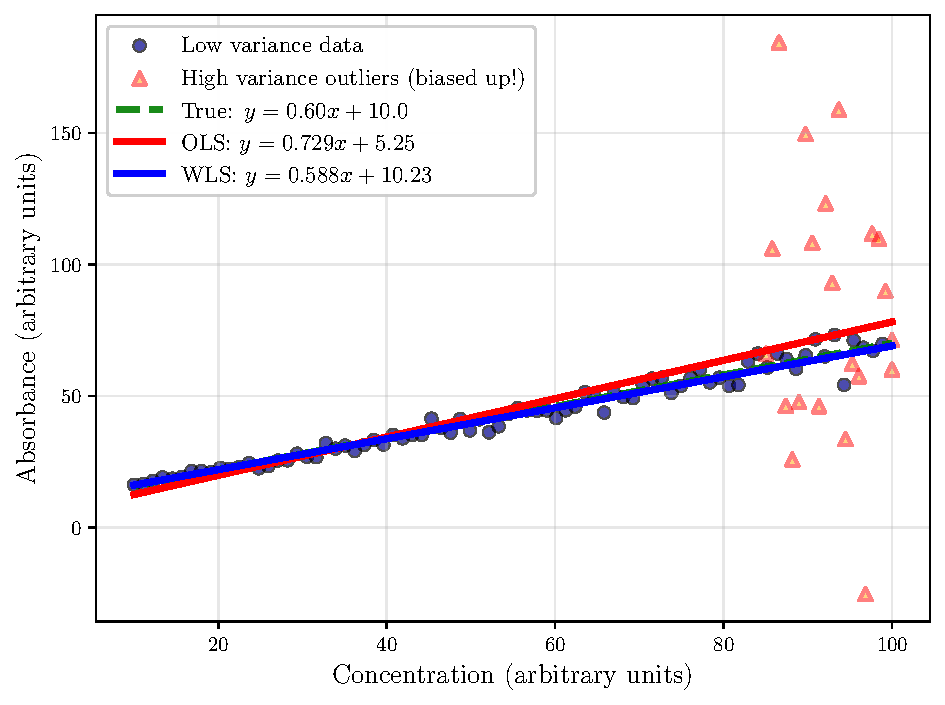
\includegraphics[width=0.6\textwidth]{figs/models-vs-data/ols_wls.pdf}
        \caption{OLS vs.\ WLS in the presence of heteroscedastic errors.}
        \label{fig:ols_wls}
    \end{figure}

    OLS treats all measurements equally, regardless of their precision. The biased high-concentration outliers heavily influence the fit, pulling the slope upward. The resulting OLS estimate has a slope of 0.729, representing a 21.5\% error from the true value of 0.600.
    
    WLS assigns weights inversely proportional to measurement variance ($w_i = 1/\sigma_i^2$), effectively down-weighting unreliable high-concentration data while trusting precise low-concentration measurements. The WLS fit yields a slope of 0.588, only 2.0\% from the true value. This is roughly 10.8 times more accurate than OLS! So we can see that when measurement precision varies systematically (heteroscedasticity), WLS provides substantially better parameter estimates by appropriately weighting each data point according to its reliability. Common sources of heteroscedastic errors include detector saturation, signal-dependent noise, and concentration-dependent matrix effects.
    
\end{exampleBox}

\subsection{Regularization}
The ordinary and weighted least squares solutions provide a direct way to find parameters that minimize the fit error. However, these methods can encounter problems, particularly when: (1) the number of features $n$ is large, approaching or exceeding the number of data points $N$; (2) the input features are highly correlated (multicollinearity), making the $\mathbf{X}^\top\mathbf{X}$ matrix ill-conditioned or singular, leading to unstable solutions; or (3) we want to encourage a simpler model, perhaps one where many parameters are exactly zero. In these situations, the OLS/WLS solution can have extremely large parameter values, leading to a model that fits the training data perfectly but performs poorly on new, unseen data (i.e., it overfits). To combat this, we introduce \textbf{regularization terms} to our objective function. These terms add a penalty for complexity, which drives the parameter estimates towards more stable and generalizable solutions.

The general idea is to modify the optimization problem to minimize not just the sum of squared errors, but also a function of the parameter magnitudes:
\begin{equation}
    \boldsymbol{\theta}^* = \arg\min_{\boldsymbol{\theta}} \left( (\mathbf{y} - \mathbf{X}\boldsymbol{\theta})^\top \mathbf{V}_{\boldsymbol{\epsilon}}^{-1} (\mathbf{y} - \mathbf{X}\boldsymbol{\theta}) + \text{Regularization Penalty} \right)
    \label{eq:regularization-general}
\end{equation}
The choice of the regularization penalty defines different types of regularized regression.

\paragraph*{L2 Regularization}
L2 regularization, also known as ridge regression, adds a penalty proportional to the sum of the squared magnitudes of the parameters. This encourages parameters to be small (i.e., it more evenly distributes the weight across all parameters) but rarely drives them exactly to zero.
\begin{equation}
    \boldsymbol{\theta}^* = \arg\min_{\boldsymbol{\theta}} (\mathbf{y} - \mathbf{X}\boldsymbol{\theta})^\top \mathbf{V}_{\boldsymbol{\epsilon}}^{-1} (\mathbf{y} - \mathbf{X}\boldsymbol{\theta}) + \beta||\boldsymbol{\theta}||_2^2
    \label{eq:l2-regularization}
\end{equation}
where $||\boldsymbol{\theta}||_2^2 = \sum_{i=1}^n \theta_i^2$ is the squared Euclidean (L2) norm of the parameter vector, and $\beta > 0$ is a tuning parameter that controls the strength of the regularization. A larger $\beta$ implies a stronger penalty on parameter magnitudes. The solution for ridge regression also has a closed form: 
\begin{equation}
    \boldsymbol{\theta}^* = (\mathbf{X}^\top\mathbf{V}_{\boldsymbol{\epsilon}}^{-1}\mathbf{X} + \beta\mathbf{I})^{-1}\mathbf{X}^\top\mathbf{V}_{\boldsymbol{\epsilon}}^{-1}\mathbf{y}
\end{equation}
where $\mathbf{I}$ is the identity matrix. The addition of $\beta\mathbf{I}$ to $\mathbf{X}^\top\mathbf{V}_{\boldsymbol{\epsilon}}^{-1}\mathbf{X}$ makes the matrix more stable and invertible (hopefully you remember that we've seen this type of trick to address ill-conditioning before in the context of iterative methods' update rules!).

\paragraph*{L1 Regularization}
L1 regularization, or lasso regression (least absolute shrinkage and selection operator), adds a penalty proportional to the sum of the absolute magnitudes of the parameters. A unique property of L1 regularization is that it tends to drive some parameters exactly to zero. This means it is effectively performing feature selection and thus giving a sparse model. The minimization problem is
\begin{equation}
    \boldsymbol{\theta}^* = \arg\min_{\boldsymbol{\theta}} (\mathbf{y} - \mathbf{X}\boldsymbol{\theta})^\top \mathbf{V}_{\boldsymbol{\epsilon}}^{-1} (\mathbf{y} - \mathbf{X}\boldsymbol{\theta}) + \alpha||\boldsymbol{\theta}||_1
    \label{eq:l1-regularization}
\end{equation}
where $||\boldsymbol{\theta}||_1 = \sum_{i=1}^n |\theta_i|$ is the L1 norm of the parameter vector, and $\alpha > 0$ controls the regularization strength. Unlike ridge regression, lasso generally does not have a closed-form solution and typically requires iterative optimization algorithms to solve.

\paragraph*{Elastic Net Regularization}
The elastic net combines both L1 and L2 regularization penalties. It encourages both small parameters (like ridge) and sparsity (like lasso).
\begin{equation}
    \boldsymbol{\theta}^* = \arg\min_{\boldsymbol{\theta}} (\mathbf{y} - \mathbf{X}\boldsymbol{\theta})^\top \mathbf{V}_{\boldsymbol{\epsilon}}^{-1} (\mathbf{y} - \mathbf{X}\boldsymbol{\theta}) + \alpha||\boldsymbol{\theta}||_1 + \beta||\boldsymbol{\theta}||_2^2
    \label{eq:elastic-net-regularization}
\end{equation}

\begin{exampleBox}
    \textbf{Example: Regularization in Action (Polynomial Regression).}
    To illustrate the effects of different regularization methods, we fit a degree-15 polynomial to 30 noisy observations from a sine function. \autoref{fig:regularization-comparison} shows the predictions (top row) and coefficient magnitudes (bottom row) for each method.

    \begin{figure}[H]
        \centering
        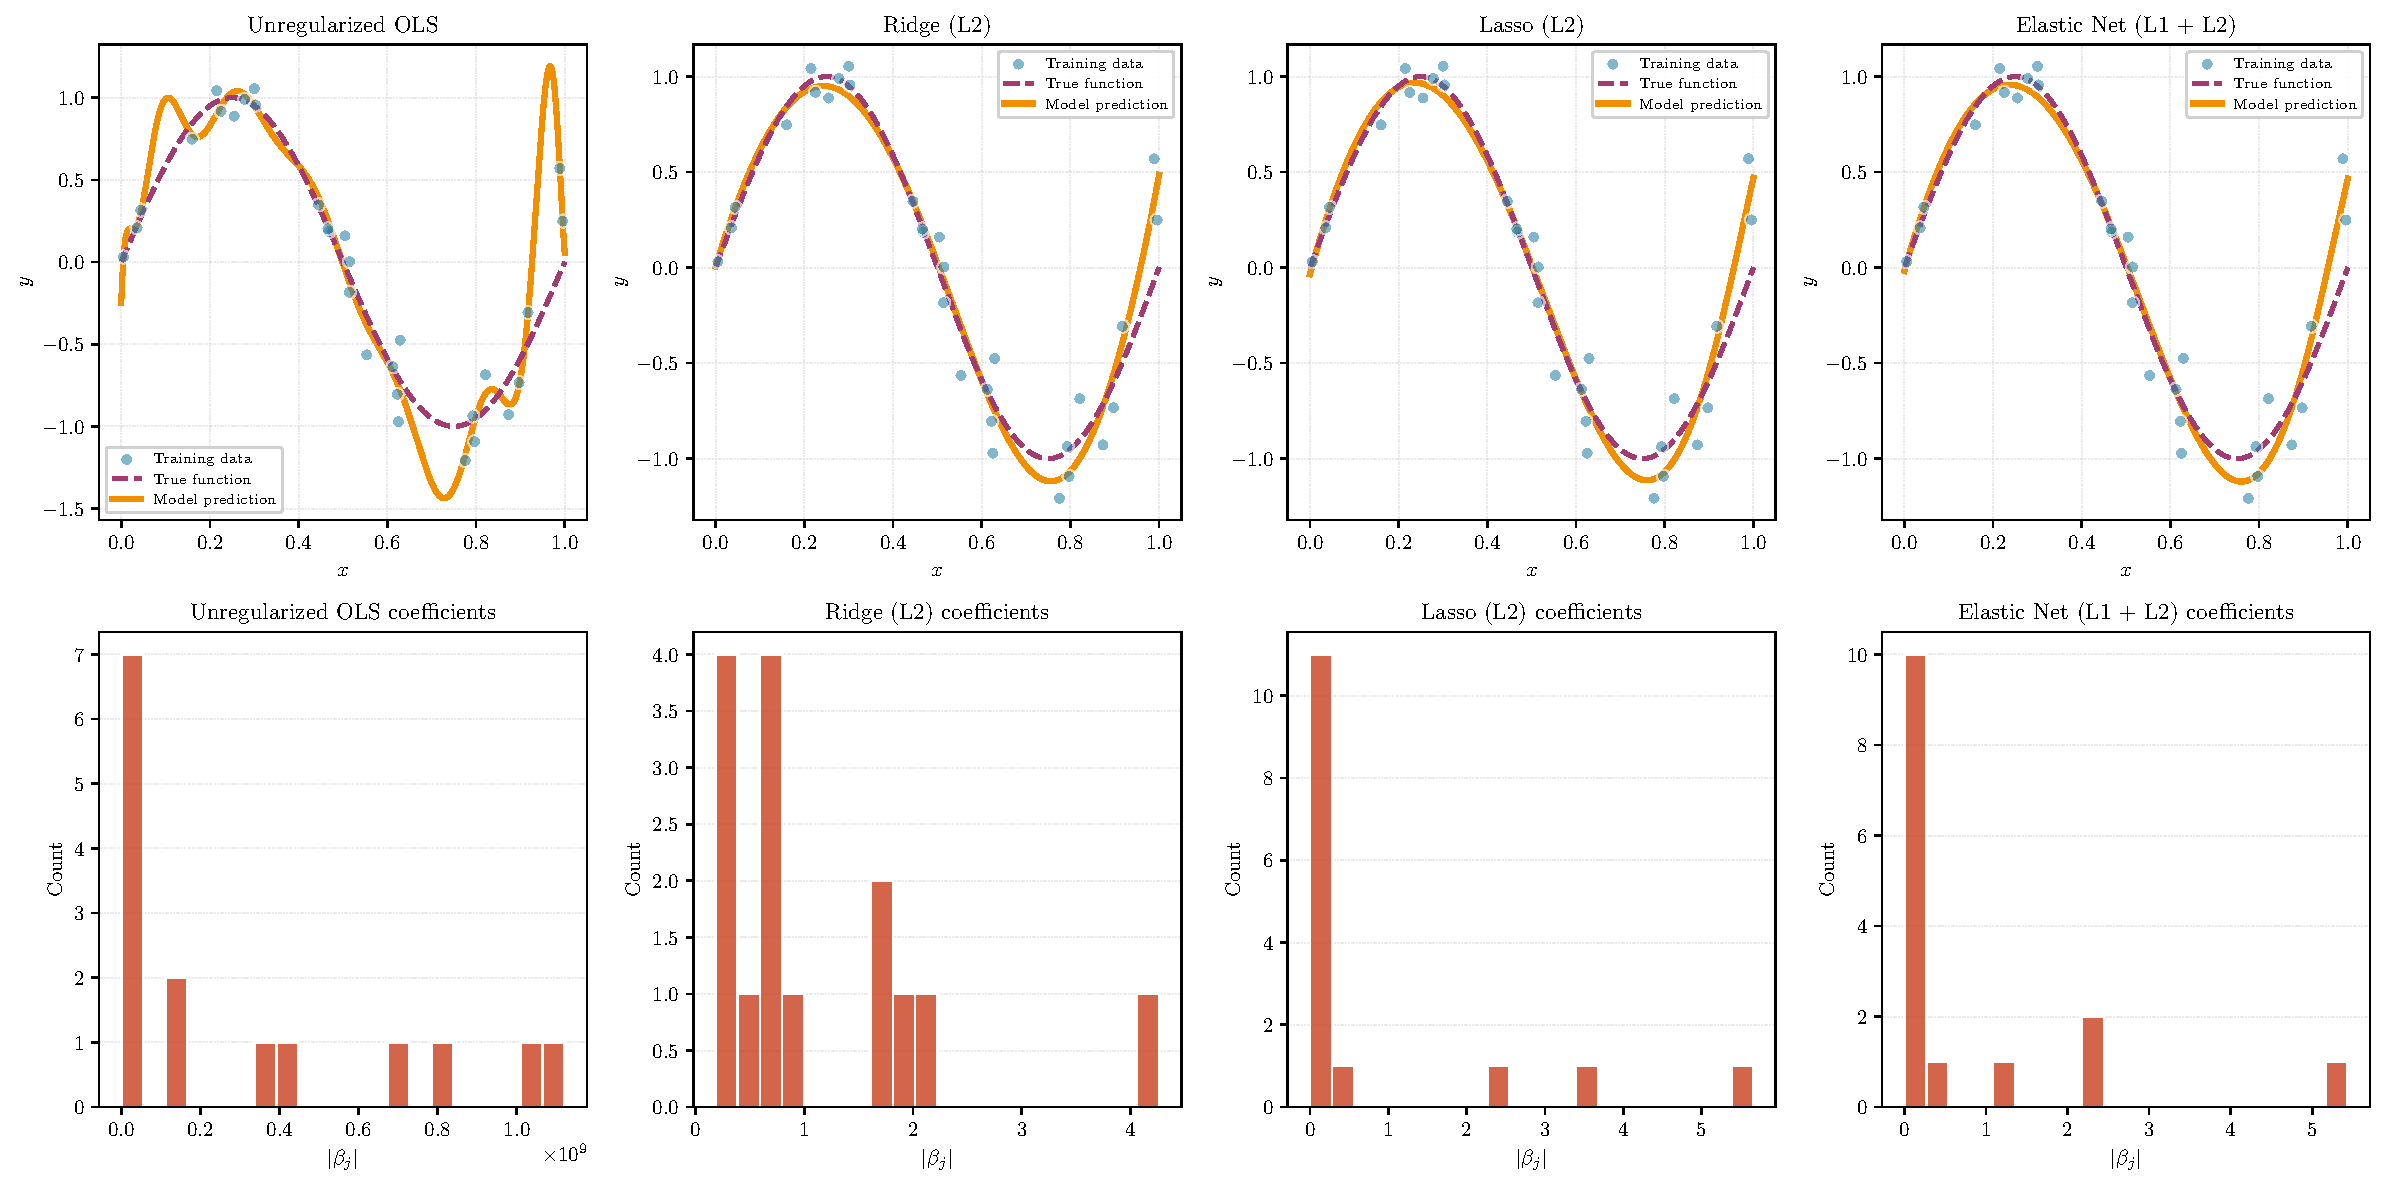
\includegraphics[width=\textwidth]{figs/models-vs-data/regularization_comparison.pdf}
        \caption{Regularization in action (polynomial regression).}
        \label{fig:regularization-comparison}
    \end{figure}
    
    \textbf{Unregularized OLS:} Without regularization, the model severely overfits the training data. Despite fitting the training points well, it exhibits wild oscillations between observations and fails to capture the true underlying function. We can see from the coefficient histogram that there are extreme parameter values (some exceeding $10^9$ in magnitude). This is typical when fitting high-degree polynomials without regularization. The ill-conditioned $\mathbf{X}^\top\mathbf{X}$ matrix leads to these pathological solutions.
    
    \textbf{Ridge (L2):} L2 regularization dramatically improves the fit. The prediction closely follows the true function with smooth interpolation between training points. The coefficient histogram shows that all parameters are shrunk to modest magnitudes, with most coefficients distributed around similar scales.
    
    \textbf{Lasso (L1):} L1 regularization also produces a smooth, accurate fit. Notably, the coefficient histogram reveals the sparsity-inducing property of lasso: the large bar at zero means that many coefficients are driven to exactly zero. Only a handful of the 15 polynomial terms are deemed necessary, so we get a simpler model.
    
    \textbf{Elastic Net (L1 + L2):} Combining both penalties, elastic net produces results similar to lasso with some coefficient sparsity, though perhaps not as aggressively as pure lasso. 

\end{exampleBox}

Above, we derived the OLS and WLS solutions by seeking the parameters that minimized the sum of squared errors. This is an intuitive and reasonable goal. However, this approach can be more rigorously justified by reframing the entire problem of parameter estimation from a probabilistic viewpoint. This is what we'll do next.

\section{Frequentist vs.\ Bayesian}
When we think about the uncertainty in model fitting, there are two dominant philosophical approaches for treating the model parameters $\boldsymbol{\theta}$. The frequentist view assumes that there is one true, fixed, but unknown parameter vector, $\boldsymbol{\theta}^*$. The data we observe, $\mathcal{D}$, is considered a random sample from a process governed by these true parameters. If we were to repeat our entire experiment, we would get different data, but the true $\boldsymbol{\theta}^*$ would remain the same. The goal of a frequentist is to devise procedures (estimators) that have good long-run properties, like being unbiased. On the other hand, the Bayesian view treats the parameters themselves as uncertain quantities. It assumes that $\boldsymbol{\theta}$ is a random vector, and we can use probability distributions to describe our degree of belief about its values.

The Bayesian approach uses Bayes' theorem to formalize the process of learning. Given our observed data $\mathcal{D}$, we update our initial beliefs about the parameters (the \textit{prior}) to arrive at an updated belief (the \textit{posterior}).
\begin{equation}
    \underbrace{p(\boldsymbol{\theta}|\mathcal{D})}_{\text{posterior}} = \frac{\overbrace{p(\mathcal{D}|\boldsymbol{\theta})}^{\text{likelihood}} \overbrace{p(\boldsymbol{\theta})}^{\text{prior}}}{\underbrace{p(\mathcal{D})}_{\text{evidence}}}
    \label{eq:bayes-theorem-annotated}
\end{equation}
We've seen this before when we introduced Bayes' theorem in the context of probability, but we'll review what each piece means here again. The prior, $p(\boldsymbol{\theta})$, reflects our beliefs about the parameters \textit{before} we see any data. The likelihood, $p(\mathcal{D}|\boldsymbol{\theta})$, is the probability of observing our specific dataset $\mathcal{D}$ if the parameters were in fact $\boldsymbol{\theta}$. The posterior, $p(\boldsymbol{\theta}|\mathcal{D})$, is our updated belief about the parameters \textit{after} observing the data. It combines our prior knowledge with the information from the data. We will now see that the concept of the likelihood is the basis of the frequentist approach to parameter estimation.

\section{Maximum Likelihood Estimation}
The most common frequentist method for parameter estimation is maximum likelihood estimation (MLE). MLE takes the simple stance that we should choose the parameters $\boldsymbol{\theta}^*$ that make our observed data $\mathcal{D}$ the most probable. In other words, we seek the parameters that maximize the likelihood function.
\begin{equation}
    \boldsymbol{\theta}_{\text{MLE}}^* = \arg\max_{\boldsymbol{\theta}} p(\mathcal{D}|\boldsymbol{\theta})
\end{equation}
Let's apply this to the linear model we've been using: $\boldsymbol{\mathsf{y}} = \mathbf{X}\boldsymbol{\theta} + \boldsymbol{\epsilon}$, where we assume the noise is drawn from a multivariate Gaussian distribution with zero mean and covariance $\mathbf{V}_{\boldsymbol{\epsilon}}$, i.e., $\boldsymbol{\epsilon} \sim \mathcal{N}(\mathbf{0}, \mathbf{V}_{\boldsymbol{\epsilon}})$. Under this assumption, the likelihood of observing our data vector $\mathbf{y}$ for a given set of parameters $\boldsymbol{\theta}$ is given by the multivariate normal PDF:
\begin{equation}
    p(\mathcal{D}|\boldsymbol{\theta}) = p(\mathbf{y}|\mathbf{X}, \boldsymbol{\theta}) = \frac{1}{(2\pi)^{N/2}|\mathbf{V}_{\boldsymbol{\epsilon}}|^{1/2}} \exp\left[-\frac{1}{2}(\mathbf{y} - \mathbf{X}\boldsymbol{\theta})^\top \mathbf{V}_{\boldsymbol{\epsilon}}^{-1}(\mathbf{y} - \mathbf{X}\boldsymbol{\theta})\right]
\end{equation}
Our goal is to find the $\boldsymbol{\theta}$ that maximizes this expression. Because the logarithm is a monotonically increasing function, maximizing a function is equivalent to maximizing its logarithm, so we can work with the log-likelihood instead. This is a lot more convenient since it turns multiplications into additions and exponentials into linear terms.
\begin{align*}
    \log p(\mathcal{D}|\boldsymbol{\theta}) &= \log \left( \frac{1}{(2\pi)^{N/2}|\mathbf{V}_{\boldsymbol{\epsilon}}|^{1/2}} \exp\left[-\frac{1}{2}(\mathbf{y} - \mathbf{X}\boldsymbol{\theta})^\top \mathbf{V}_{\boldsymbol{\epsilon}}^{-1}(\mathbf{y} - \mathbf{X}\boldsymbol{\theta})\right] \right) \\
    &= -\frac{N}{2}\log(2\pi) - \frac{1}{2}\log|\mathbf{V}_{\boldsymbol{\epsilon}}| - \frac{1}{2}(\mathbf{y} - \mathbf{X}\boldsymbol{\theta})^\top \mathbf{V}_{\boldsymbol{\epsilon}}^{-1}(\mathbf{y} - \mathbf{X}\boldsymbol{\theta})
\end{align*}
To find the optimal $\boldsymbol{\theta}$, we can discard any terms that do not depend on it, giving us
\begin{equation}
    \boldsymbol{\theta}_{\text{MLE}}^* = \arg\max_{\boldsymbol{\theta}} \left[ -\frac{1}{2}(\mathbf{y} - \mathbf{X}\boldsymbol{\theta})^\top \mathbf{V}_{\boldsymbol{\epsilon}}^{-1}(\mathbf{y} - \mathbf{X}\boldsymbol{\theta}) \right]
\end{equation}
Maximizing a negative quantity is the same as minimizing its positive counterpart, and we can throw away the prefactor of $1/2$ since it doesn't change the location of the minimum. Therefore, the MLE solution is
\begin{equation}
    \boldsymbol{\theta}_{\text{MLE}}^* = \arg\min_{\boldsymbol{\theta}} \left[ (\mathbf{y} - \mathbf{X}\boldsymbol{\theta})^\top \mathbf{V}_{\boldsymbol{\epsilon}}^{-1}(\mathbf{y} - \mathbf{X}\boldsymbol{\theta}) \right]
\end{equation}
This is precisely the objective function for WLS! So the intuitive method of minimizing the sum of squared errors is equivalent to the more formal method of MLE provided that we assume the experimental noise is independent and Gaussian. This gives a nice probabilistic justification for the widespread use of least-squares methods.

\section{Maximum a Posteriori Estimation}
The MLE approach assumes there is one true parameter set that we are trying to find. By contrast, the Bayesian approach allows for uncertainty in the parameters themselves by treating them as random variables. This lets us incorporate our own prior knowledge or beliefs into the estimation process. While a full Bayesian analysis involves finding the entire posterior distribution $p(\boldsymbol{\theta}|\mathcal{D})$, we often want a single point estimate for the parameters. The Bayesian equivalent of the MLE is the \textbf{maximum a posteriori (MAP)} estimate, which seeks the most probable parameter vector \textit{given the data}. In other words, we find the peak, or mode, of the posterior distribution.
\begin{equation}
    \boldsymbol{\theta}_{\text{MAP}}^* = \arg\max_{\boldsymbol{\theta}} p(\boldsymbol{\theta}|\mathcal{D})
\end{equation}
Using Bayes' theorem, we can rewrite this as
\begin{equation}
    \boldsymbol{\theta}_{\text{MAP}}^* = \arg\max_{\boldsymbol{\theta}} \frac{p(\mathcal{D}|\boldsymbol{\theta})p(\boldsymbol{\theta})}{p(\mathcal{D})}
\end{equation}
Since the evidence term $p(\mathcal{D})$ in the denominator does not depend on our parameters $\boldsymbol{\theta}$, it doesn't affect the location of the maximum. We can therefore simplify the optimization problem to maximizing the numerator:
\begin{equation}
    \boldsymbol{\theta}_{\text{MAP}}^* = \arg\max_{\boldsymbol{\theta}} p(\mathcal{D}|\boldsymbol{\theta})p(\boldsymbol{\theta})
\end{equation}
The difference between MLE and MAP is just one term, the prior distribution $p(\boldsymbol{\theta})$. MLE maximizes only the likelihood, whereas MAP maximizes the likelihood multiplied by the prior.

\paragraph*{The Role of the Prior}
The prior distribution $p(\boldsymbol{\theta})$ is our way of encoding beliefs about the parameters \textit{before} observing any data. This knowledge might come from physical laws, previous experiments, or expert opinion. The resulting posterior distribution is a principled compromise between our prior beliefs and the evidence from the new data.

\begin{figure}[h!]
    \centering
    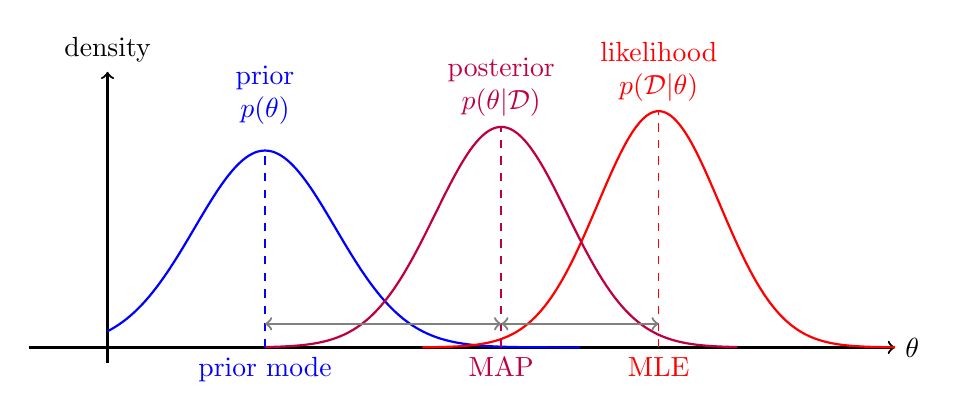
\begin{tikzpicture}
        \draw[->,thick] (-1,0) -- (10,0) node[right] {$\theta$};
        \draw[->,thick] (0,-0.2) -- (0,3.5) node[above] {density};
        
        \draw[blue, thick, domain=0:6, samples=100, smooth] 
            plot (\x, {2.5*exp(-0.5*(\x-2)^2/0.8)});
        \node[blue, align=center] at (2, 3.2) {prior\\ $p(\theta)$};
        
        \draw[red, thick, domain=4:10, samples=100, smooth] 
            plot (\x, {3*exp(-0.5*(\x-7)^2/0.6)});
        \node[red, align=center] at (7, 3.5) {likelihood \\ $p(\mathcal{D}|\theta)$};
        
        \draw[purple, thick, domain=2:8, samples=100, smooth] 
            plot (\x, {2.8*exp(-0.5*(\x-5)^2/0.7)});
        \node[purple, align=center] at (5, 3.3) {posterior\\ $p(\theta|\mathcal{D})$};
        
        \draw[blue, dashed, thin] (2,0) -- (2,2.5) node[below, yshift=-2.5cm] {prior mode};
        \draw[red, dashed, thin] (7,0) -- (7,3.0) node[below, yshift=-3cm] {MLE};
        \draw[purple, dashed, thick] (5,0) -- (5,2.8) node[below, yshift=-2.8cm] {MAP};
        
        \draw[<->, thick, gray] (2,0.3) -- (5,0.3) node[midway, above, font=\small] {};
        \draw[<->, thick, gray] (5,0.3) -- (7,0.3) node[midway, above, font=\small] {};
        
    \end{tikzpicture}
    \caption{The relationship between prior, likelihood, and posterior. The posterior distribution's peak (the MAP estimate) is a compromise, pulled away from the likelihood's peak by the influence of the prior.}
    \label{fig:prior-likelihood-posterior}
\end{figure}

The strength of the prior matters. A broad, uninformative prior (e.g., a uniform distribution) suggests we have little initial knowledge, and the posterior will be dominated by the data (the likelihood). A narrow, strong prior suggests we are very confident in our initial belief, and it will take a large amount of contradictory data to change our minds.

\begin{exampleBox}
    \textbf{Example: How Prior Beliefs Shape What We Learn from Data}
    
    Imagine you find a coin and flip it $N=20$ times, observing $k=12$ heads (60\% heads). Is this coin fair, or is it biased? Your answer depends not just on what you observed, but also on what you believed \emph{before} seeing the data. The data alone (12 heads in 20 flips) suggests the coin favors heads, with peak likelihood around $\theta \approx 0.6$. But should we trust this conclusion fully? Let's consider three different starting points. We'll omit the explicit calculations of the posteriors here for brevity and simply state the results in each case.\footnote{Check out the optional section on conjugate priors for some extra info on the particular class of distribution chosen for our modeling here!}
    
    First, suppose you know nothing about this coin. You adopt a uniform prior Beta$(1,1)$, which assigns equal probability to any value of $\theta$ from 0 to 1. You're saying: ``I have no reason to favor any hypothesis over another.'' In this case, the posterior Beta$(13,9)$ closely follows the data, concentrating around $\theta \approx 0.6$. With weak prior beliefs, the data dominates your conclusion. This is shown in \autoref{fig:coin-priors} (A).
    
    Now, suppose you have strong reason to believe the coin is fair; perhaps it's a fresh coin from the national mint, where quality control is rigorous. You encode this belief with Beta$(20,20)$, a prior that strongly expects $\theta \approx 0.5$. Even after seeing 12 heads, your posterior Beta$(32,28)$ remains centered near fairness (approximately 0.53), only slightly nudged by the data. Strong, well-justified priors act as regularizers, preventing you from overreacting to moderate evidence. This skepticism is valuable when you have domain knowledge suggesting the data might be noisy or sample sizes small. This is shown in \autoref{fig:coin-priors} (B).
    
    Finally, suppose you suspect this coin is heavily biased toward heads; perhaps someone told you it was a trick coin. You start with Beta$(8,2)$, centered around $\theta \approx 0.8$. Now, your posterior Beta$(20,10)$ is a compromise: the data pulled you down from 0.8 toward 0.6, but you haven't fully accepted the data's verdict. You end up around $\theta \approx 0.67$. Misspecified priors can bias your conclusions, anchoring you away from what the data actually shows. This is both a feature (if your prior knowledge is genuine) and a bug (if your prior is wrong). This is shown in \autoref{fig:coin-priors} (C).
    
    Bayesian inference is a negotiation between prior beliefs and observed data. Weak priors let the data speak loudly, while strong priors demand more evidence before changing your mind. The art lies in choosing priors that honestly reflect your knowledge (or lack thereof) before seeing the data.
    
    \begin{figure}[H]
        \centering
        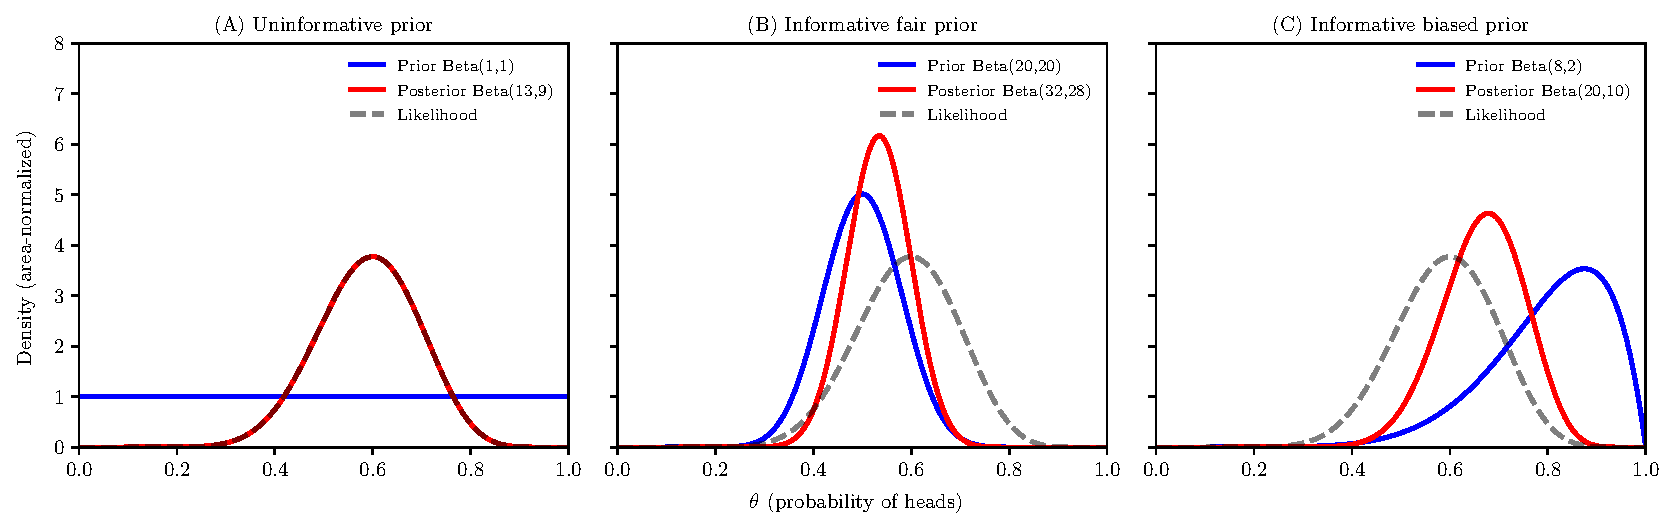
\includegraphics[width=\textwidth]{figs/models-vs-data/coin_priors_subplots.pdf}
        \caption{The effect of the prior on the posterior for a coin-toss experiment (12 heads, 8 tails out of 20 flips). Each panel shows how different prior beliefs (blue) combine with the same likelihood (dashed) to produce different posteriors (red).}
        \label{fig:coin-priors}
    \end{figure}
\end{exampleBox}
    

\paragraph*{Priors as Regularization}
The connection between priors and the regularization techniques we saw earlier is one of the most elegant results in statistical modeling. Let's reconsider our linear model fitting, but this time from a MAP perspective. The log of the posterior is
\begin{equation}
\log p(\boldsymbol{\theta}|\mathcal{D}) = \log p(\mathcal{D}|\boldsymbol{\theta}) + \log p(\boldsymbol{\theta}) + \text{constant} \end{equation}
Maximizing the posterior is equivalent to maximizing the log-likelihood plus the log-prior. Now, let's assume a zero-mean Gaussian prior on our parameters, $\boldsymbol{\theta} \sim \mathcal{N}(\mathbf{0}, \mathbf{I}/\beta)$. This prior encodes a belief that parameter values are more likely to be small than large. The log of this prior is
\begin{equation}
    \log p(\boldsymbol{\theta}) = -\frac{\beta}{2}\boldsymbol{\theta}^\top\boldsymbol{\theta} + \text{constant}
\end{equation}
Substituting this and the log-likelihood into the MAP objective gives
\begin{equation}
    \boldsymbol{\theta}_{\text{MAP}}^* = \arg\max_{\boldsymbol{\theta}} \left( -\frac{1}{2}(\mathbf{y} - \mathbf{X}\boldsymbol{\theta})^\top \mathbf{V}_{\boldsymbol{\epsilon}}^{-1}(\mathbf{y} - \mathbf{X}\boldsymbol{\theta}) - \frac{\beta}{2}\boldsymbol{\theta}^\top\boldsymbol{\theta} \right)
\end{equation}
Maximizing this is equivalent to minimizing its negative, so
\begin{equation}
    \boldsymbol{\theta}_{\text{MAP}}^* = \arg\min_{\boldsymbol{\theta}} \left( (\mathbf{y} - \mathbf{X}\boldsymbol{\theta})^\top \mathbf{V}_{\boldsymbol{\epsilon}}^{-1}(\mathbf{y} - \mathbf{X}\boldsymbol{\theta}) + \beta\boldsymbol{\theta}^\top\boldsymbol{\theta} \right)
\end{equation}
This is exactly the objective function for L2 regularization (ridge regression)! So we have a Bayesian interpretation for regularization: it is equivalent to MAP estimation with a prior belief that the parameters should be small and centered around zero. A similar result holds for L1 regularization using a Laplace prior.

\section{The Chi-Square Statistic}
We have established that for a linear model with Gaussian noise, the MLE is equivalent to the WLS solution. This procedure gives us the single ``best'' set of parameters, $\boldsymbol{\theta}^*$, that minimizes the discrepancy between our model's predictions and the observed data. However, finding the best-fit parameters does not tell us if the fit is actually any good. The model might be fundamentally wrong (imagine fitting a line to a parabolic dataset), yet our optimization will still dutifully find the parameter values that make this bad model look as good as possible. We need a way to step back and ask a more fundamental question: Is the data consistent with the model itself, even with its optimal parameters? We have already encountered the necessary tool to answer this. When we assumed Gaussian noise to derive the MLE solution, we sought to minimize the quantity in the exponent of the likelihood function. This quantity is so fundamental to goodness-of-fit testing that it is given its own name: the \textbf{chi-square} ($\chi^2$) statistic.
\begin{equation}
    \chi^2 = (\mathbf{y} - \tilde{\mathbf{y}}(\mathbf{X}; \boldsymbol{\theta}))^\top \mathbf{V}_{\boldsymbol{\epsilon}}^{-1} (\mathbf{y} - \tilde{\mathbf{y}}(\mathbf{X}; \boldsymbol{\theta}))
\end{equation}
Here, $\tilde{\mathbf{y}}(\mathbf{X}; \boldsymbol{\theta})$ represents the model's predictions using a specific set of parameters $\boldsymbol{\theta}$. Finding the maximum likelihood estimate, $\boldsymbol{\theta}_{\text{MLE}}^*$, is therefore entirely equivalent to finding the parameters that \textit{minimize} the chi-square value: $\boldsymbol{\theta}_{\text{MLE}}^* = \arg\min_{\boldsymbol{\theta}} \chi^2$.

The $\chi^2$ value has an intuitive meaning. If the noise is uncorrelated so that the covariance matrix $\mathbf{V}_{\boldsymbol{\epsilon}}$ is diagonal with entries $[\mathbf{V}_{\boldsymbol{\epsilon}}]_{ii} = \sigma_i^2$, the expression simplifies to a sum:
\begin{equation}
    \chi^2 = \sum_{i=1}^N \frac{(y_i - \tilde{y}(\mathbf{x}_i; \boldsymbol{\theta}))^2}{\sigma_i^2}
    \label{eq:chi-square-sum}
\end{equation}
This is the sum of squared residuals where each residual is normalized by the variance of its corresponding measurement. It measures the discrepancy between the data and the model in units of the expected statistical error. If the model is a good fit, we would expect the typical deviation $(y_i - \tilde{y}_i)$ to be on the order of the standard deviation $\sigma_i$. Thus, each term in the sum should be roughly equal to one, and we would expect the total $\chi^2$ value to be approximately equal to the number of degrees of freedom, $\nu = N - n$, where $n$ is the number of fitted parameters.

\begin{warningBox}
    \textbf{Known vs.\ Estimated Error Variances}

    In this treatment, we assume the error covariance matrix $\mathbf{V}_{\boldsymbol{\epsilon}}$ (or equivalently, the individual error variances $\sigma_i^2$) is known a priori from prior calibration, repeated measurements, or theoretical considerations. Under this assumption, the MLE/WLS estimate $\boldsymbol{\theta}^*_{\text{MLE}}$ minimizes $\chi^2$, and for linear models, $\chi^2(\boldsymbol{\theta}^*_{\text{MLE}})$ follows a $\chi^2_{N-n}$ distribution exactly. If instead the errors have an unknown common scale $\sigma^2$ (e.g., $\sigma_i^2 = \sigma^2 w_i$ with known weights $w_i$), then $\sigma^2$ must also be estimated from the data. In this case, the MLE simultaneously estimates both $\boldsymbol{\theta}$ and $\sigma^2$. The distribution of the rescaled residuals changes: $\chi^2/\hat{\sigma}^2$ follows different distributions (related to Student's t and F distributions), and the expectation of $\chi^2_\nu$ is slightly below 1. The methods we develop here still apply, but interpretation of goodness-of-fit (discussed later on) requires care. Throughout this text, we assume $\mathbf{V}_{\boldsymbol{\epsilon}}$ is known unless stated otherwise.
\end{warningBox}

\subsection{The Chi-Square Distribution and Hypothesis Testing}
Much of the utility of the $\chi^2$ statistic comes from recognizing that it can be treated as a random variable. If our model is indeed correct, and we were to repeat the experiment, we would obtain a new data vector $\mathbf{y}$ due to random noise, which in turn would yield a new, slightly different $\chi^2$ value. The distribution of these possible $\chi^2$ values, under the assumption that the model is correct, is known as the \textbf{chi-square distribution}. Its PDF (visualized in the leftmost panel of \autoref{fig:chi2-distributions}) is given by
\begin{equation}
    p_{\chi^2}(\chi^2; \nu) = \frac{1}{2^{\nu/2}\Gamma(\nu/2)} e^{-\chi^2/2} (\chi^2)^{(\nu/2)-1}
\end{equation}
The chi-square distribution arises naturally in this context. Under our assumptions of Gaussian noise, each normalized residual $(y_i - \tilde{y}_i)/\sigma_i$ is a standard normal random variable. The $\chi^2$ statistic is a sum of the squares of such variables (accounting for correlations through $\mathbf{V}_{\boldsymbol{\epsilon}}^{-1}$). When these residuals are independent and we evaluate at the fitted parameters, this sum follows a chi-square distribution with $\nu$ degrees of freedom.
\begin{figure}[h!]
    \centering
    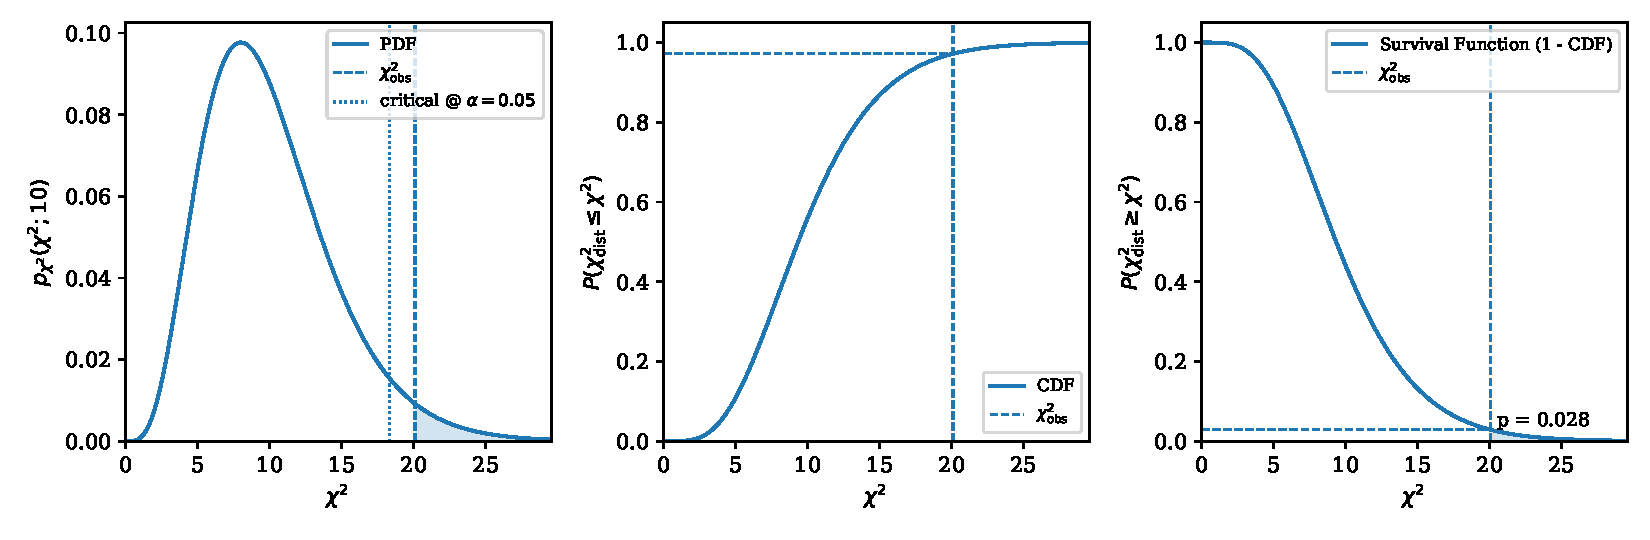
\includegraphics[width=\textwidth]{figs/models-vs-data/chi_square.pdf}
    \caption{The chi-square distribution for $\nu=10$ degrees of freedom. The PDF (left) shows the probability density for any given $\chi^2$ value. The CDF (center) shows the cumulative probability $P(\chi^2_{\text{dist}} \le \chi^2)$. The survival function (right), or $1-\text{CDF}$, directly gives the \textbf{upper-tail p-value} corresponding to an observed $\chi^2$ value. The shaded region illustrates $p = P(\chi^2_{10} \ge \chi^2_{\text{obs}})$ for a hypothetical observed value.}
    \label{fig:chi2-distributions}
\end{figure}
\begin{warningBox}
    \textbf{Warning:} The $\chi^2$ distribution is only valid under specific conditions: (1) the model structure is correct, (2) the measurement errors are truly Gaussian distributed, (3) the error estimates ($\sigma_i$ or $\mathbf{V}_{\boldsymbol{\epsilon}}$) are accurate, and (4) the errors are independent (or their correlations are correctly specified in $\mathbf{V}_{\boldsymbol{\epsilon}}$). Violations of these assumptions can lead to unreliable p-values and incorrect conclusions about model fit.

    Additionally, for linear models with known $\mathbf{V}_{\boldsymbol{\epsilon}}$, the distribution $\chi^2(\boldsymbol{\theta}^*_{\text{MLE}}) \sim \chi^2_{N-n}$ is exact. For nonlinear models, this result is \textit{asymptotic} (valid for large $N$). With small sample sizes or highly nonlinear models, the actual sampling distribution may deviate from $\chi^2_{N-n}$, leading to unreliable p-values.
\end{warningBox}
As mentioned, this distribution is defined by a single parameter, $\nu$, called the degrees of freedom. The degrees of freedom represent the number of independent pieces of information available for assessing the model's fit. When evaluating $\chi^2$ at the MLE parameters $\boldsymbol{\theta}^*$, it is calculated as the number of data points ($N$) minus the number of parameters ($n$) that were estimated from the data:
\begin{equation}
    \nu = N - n
\end{equation}
Intuitively, each time we use the data to estimate a parameter (like a slope or an intercept), we spend one degree of freedom. That parameter is now tuned to fit the data, so the data is no longer completely free to vary. The remaining degrees of freedom, $\nu$, reflect how much the data is still free to challenge the model's overall structure.

This framework allows us to perform a formal hypothesis test. Our null hypothesis, $H_0$, is that our model is a correct description of the data-generating process. We then ask, ``Assuming our model is correct, what is the probability that random chance would produce a $\chi^2$ value at least as large as the one we actually observed?'' This probability is the \textbf{p-value}. A very small p-value implies that our observed data is highly unlikely under the model (i.e., the model is probably a poor fit).

To find the p-value, we compute the upper-tail probability: the probability that a $\chi^2$ random variable with $\nu$ degrees of freedom would equal or exceed our observed value. This is $p = P(\chi^2_\nu \ge \chi^2_{\text{obs}}) = 1 - \text{CDF}(\chi^2_{\text{obs}})$, which is shown as the survival function in the rightmost panel of \autoref{fig:chi2-distributions}. Before running the experiment, we decide on a significance level, $\alpha$, typically 0.05. If our calculated p-value is less than $\alpha$, we reject the null hypothesis and conclude that the data provides statistically significant evidence against the model. For example, with $\nu=10$ degrees of freedom, the critical value (upper $(1-\alpha)$ quantile) corresponding to $\alpha=0.05$ is $\chi^2_{\text{inv}}(0.95, 10) = 18.307$. This means there is only a 5\% chance of observing $\chi^2 \ge 18.307$ if the model is correct. If our experiment yielded $\chi^2_{\text{obs}} = 20.1$, our p-value would be less than 0.05, and we would reject the model.

\begin{warningBox}
    \textbf{Warning:} We should be careful to correctly interpret the p-value. If we calculate $p=0.03$, it means there is a 3\% chance of observing data at least this discrepant \textit{if the model were true}. It does \textbf{not} mean there is a 3\% chance the model is correct or a 97\% chance the model is false. The p-value is a statement about the probability of the data conditional on the model, not the other way around.
\end{warningBox}

\paragraph*{The Reduced Chi-Square}
A useful rule of thumb in practice is the \textbf{reduced chi-square}, defined as $\chi^2_\nu = \chi^2 / \nu$. For a linear model with known error covariance $\mathbf{V}_{\boldsymbol{\epsilon}}$, we have $\mathbb{E}[\chi^2(\boldsymbol{\theta}^*_{\text{MLE}})] = \nu$, so we expect $\chi^2_\nu \approx 1$ for a good fit. A large value ($\chi^2_\nu \gg 1$) suggests a poor model fit: the discrepancy between the data and the model is significantly larger than what the measurement noise would justify. Conversely, a value much less than one ($\chi^2_\nu \ll 1$) is also problematic and can indicate several issues: the model may be overfitting the data (too many free parameters relative to the information content), the measurement errors ($\sigma_i$) have been systematically overestimated, or there may be correlations in the noise that have not been properly accounted for. 

\paragraph*{Notation: Chi-Square Quantiles}
Throughout this text, we use $\chi^2_{\text{inv}}(1-\alpha, \nu)$ to denote the upper $(1-\alpha)$ quantile of the chi-square distribution with $\nu$ degrees of freedom. This is the critical value $c$ such that $P(\chi^2_\nu \le c) = 1-\alpha$, or equivalently, $P(\chi^2_\nu \ge c) = \alpha$. For example, $\chi^2_{\text{inv}}(0.95, 1) = 3.84$ means 95\% of $\chi^2_1$ values fall below 3.84, and $\chi^2_{\text{inv}}(0.95, 10) = 18.31$ means 95\% of $\chi^2_{10}$ values fall below 18.31. (Be aware that some texts or papers use notation like $\chi^2_{\alpha,\nu}$ or $\chi^2_{\nu}(\alpha)$ for the same concept.)


% MC: the slides only discuss the absolute criterion approach, not the likelihood ratio approach
% but we should probably cover both, especially because students who ask LLMs for help will get
% very confused. also, my understanding is that the likelihood approach is the best
\section{Regions of Indifference}
With the above chi-square goodness-of-fit test, we have laid the groundwork for defining a \textbf{region of indifference}, which is the set of all parameter vectors $\boldsymbol{\theta}$ that agree ``well enough'' with our data. The question of what constitutes ``well enough'' can be answered in two different ways, each with its own statistical interpretation and practical implications. Both approaches use the chi-square distribution but differ in their philosophical stance on what we're testing.

\begin{definitionBox}
\textbf{Two Approaches to Confidence Regions}

\textit{The Absolute Fit Approach:} We might ask, ``Which parameter values would produce a model that we would not reject as inconsistent with the data?'' This leads us to define the confidence region as all parameter vectors $\boldsymbol{\theta}$ where the chi-square goodness-of-fit test does not reject the model. Formally, given a significance level $\alpha$, this is
\begin{equation}
    \{\boldsymbol{\theta} \ : \ \chi^2(\boldsymbol{\theta}) \leq \chi^2_{\text{inv}}(1-\alpha, N-n)\}
\end{equation}
where $N-n$ are the degrees of freedom from the goodness-of-fit test ($N$ observations, $n$ parameters). This approach is conservative and guarantees that any parameter vector in this region corresponds to an acceptable fit to the data. However, the size of this confidence region depends on how well the best-fit model performs: better-fitting models give larger confidence regions.

\textit{The Likelihood Ratio Approach:} Alternatively, we might ask, ``How much can the parameters deviate from their maximum likelihood estimates before the degradation in fit becomes statistically significant?'' This perspective focuses on the \textit{change} in fit quality rather than the absolute fit. Under this approach, the confidence region consists of parameter values where
\begin{equation}
    \Delta\chi^2 = \chi^2(\boldsymbol{\theta}) - \chi^2(\boldsymbol{\theta}^*_{\text{MLE}}) \leq \chi^2_{\text{inv}}(1-\alpha, n)
\end{equation}
where now the degrees of freedom equal the number of parameters $n$. This is the standard method in likelihood-based inference\footnote{This approach comes from Wilks' theorem on the asymptotic distribution of the likelihood ratio statistic; check out the Wikipedia page on Wilk's theorem for more details.}. The confidence region size is independent of overall fit quality and depends only on the local curvature of the $\chi^2$ surface near the minimum; this is a very nice property to have!

\vspace{0.2cm}

Both approaches are mathematically valid and define ellipsoidal confidence regions (in the linear approximation), but they answer different questions and are appropriate for different purposes. The absolute fit approach is useful when we want to ensure any parameter set in our confidence region produces a model that passes a goodness-of-fit test. The likelihood ratio approach is the standard choice for quantifying parameter uncertainty in modern statistical practice, as it provides a direct connection to hypothesis testing via the likelihood ratio test and produces confidence intervals with the familiar interpretation independent of overall model fit quality. In what follows, we develop the theory using the absolute fit approach. The likelihood ratio approach follows identically by simply changing the threshold from $\chi^2_{\text{inv}}(1-\alpha, N-n)$ to $\chi^2_{\text{inv}}(1-\alpha, n)$ and measuring from $\chi^2(\boldsymbol{\theta}^*_{\text{MLE}})$ rather than from zero.
\end{definitionBox}
For convenience, we define $\chi^2_{\text{max}}$ as the threshold value in each approach: for the absolute fit approach, $\chi^2_{\text{max}} = \chi^2_{\text{inv}}(1-\alpha, N-n)$ and for the likelihood ratio approach, $\chi^2_{\text{max}} = \chi^2(\boldsymbol{\theta}^*_{\text{MLE}}) + \chi^2_{\text{inv}}(1-\alpha, n)$. As mentioned, both approaches lead to ellipsoidal confidence regions with identical local geometry and differ only in the threshold value used to define the boundary.

\begin{warningBox}
    \textbf{Important Prerequisite: Model Goodness-of-Fit}
    
    A prerequisite for constructing meaningful confidence regions is that the model must first pass a goodness-of-fit test. If $\chi^2(\boldsymbol{\theta}^*_{MLE})$ itself is unacceptably large (p-value $< \alpha$ using $\nu = N-n$ degrees of freedom), then the model is fundamentally inconsistent with the data. In this case, constructing confidence regions for the model's parameters is not meaningful, and we should reject the model entirely, not attempt to quantify uncertainty in its parameters.
    
    An important edge case arises when using the absolute fit approach: if $\chi^2(\boldsymbol{\theta}^*_{MLE})$ exceeds $\chi^2_{\text{inv}}(1-\alpha, N-n)$, the confidence region would be empty. This is a strong signal that even the most optimal parameterization of our model is statistically inconsistent with the data. Under the absolute fit criterion, there is also a subtle issue that as $\chi^2(\boldsymbol{\theta}^*_{MLE})$ approaches but does not exceed $\chi^2_{\text{inv}}(1-\alpha, N-n)$, the confidence region shrinks toward a single point. This means that marginally acceptable models (those that barely pass the goodness-of-fit test) have extremely small confidence regions, even though they satisfy the statistical criterion for model acceptance. This counterintuitive behavior is avoided in the likelihood ratio approach.
\end{warningBox}

Assuming the model passes this basic sanity check of goodness-of-fit, we now want to characterize the \textit{shape} and \textit{size} of this confidence region near the best-fit point, $\boldsymbol{\theta}^*_{MLE}$. Regardless of which approach we choose (absolute fit or likelihood ratio), the local geometry of the confidence region is determined by the curvature of the $\chi^2$ surface. To understand how $\chi^2$ varies as we move a small distance away from the minimum, we use a Taylor series expansion:
\begin{equation}
    \chi^2(\boldsymbol{\theta}) \approx \chi^2(\boldsymbol{\theta}^*_{MLE}) + (\boldsymbol{\theta} - \boldsymbol{\theta}^*_{MLE})^\top \frac{\partial \chi^2}{\partial \boldsymbol{\theta}} \bigg|_{\boldsymbol{\theta}^*_{MLE}} + \frac{1}{2}(\boldsymbol{\theta} - \boldsymbol{\theta}^*_{MLE})^\top \frac{\partial^2 \chi^2}{\partial \boldsymbol{\theta}^2} \bigg|_{\boldsymbol{\theta}^*_{MLE}} (\boldsymbol{\theta} - \boldsymbol{\theta}^*_{MLE}) + \dots
\end{equation}
Since $\boldsymbol{\theta}^*_{MLE}$ is the minimum of the $\chi^2$ surface, the first derivative (the gradient) is zero. Letting $\Delta\boldsymbol{\theta} = \boldsymbol{\theta} - \boldsymbol{\theta}^*_{MLE}$, the change in $\chi^2$ is dominated by the second-order term involving the Hessian matrix (the matrix of second partial derivatives). For a linear model, this expansion is exact. For nonlinear models, this is an excellent approximation near the minimum, where higher-order terms are negligible. The Hessian of the $\chi^2$ statistic can be calculated. For the general case with non-independent observations, where $\chi^2(\boldsymbol{\theta}) = \sum_{i=1}^N \sum_{j=1}^N (y_i - \tilde{y}(\mathbf{x}_i; \boldsymbol{\theta}))[\mathbf{V}_\epsilon^{-1}]_{ij}(y_j - \tilde{y}(\mathbf{x}_j; \boldsymbol{\theta}))$, the Hessian is approximately:
\begin{equation}
    \frac{\partial^2 \chi^2}{\partial \theta_k \partial \theta_l} \approx 2 \sum_{i=1}^N \sum_{j=1}^N \frac{\partial \tilde{y}}{\partial \theta_k}\bigg|_{\mathbf{x}=\mathbf{x}_i} [\mathbf{V}_\epsilon^{-1}]_{ij} \frac{\partial \tilde{y}}{\partial \theta_l}\bigg|_{\mathbf{x}=\mathbf{x}_j}
    \label{eq:hessian-approx}
\end{equation}
\begin{theoremBox}
    \textbf{The Gauss-Newton Approximation to the Hessian}
    
    The expression in \autoref{eq:hessian-approx} for the Hessian is an approximation known as the Gauss-Newton matrix. The complete second derivative of $\chi^2$ includes an additional term:
    \begin{equation}
        \frac{\partial^2 \chi^2}{\partial \theta_k \partial \theta_l} = 2\mathbf{J}^\top \mathbf{V}_\epsilon^{-1} \mathbf{J} - 2\sum_{i=1}^N \sum_{j=1}^N (y_i - \tilde{y}_i)[\mathbf{V}_\epsilon^{-1}]_{ij} \frac{\partial^2 \tilde{y}_j}{\partial \theta_k \partial \theta_l}
    \end{equation}
    The second term involves both second derivatives of the model (which vanish for linear models) and the residuals $(y_i - \tilde{y}_i)$. This term is almost universally neglected in practice for several reasons. First, its expectation is zero: if the model is correct, the residuals are noise with zero mean, so this term averages to zero over many realizations of the data. Second, it is dominated by the first term near the MLE when residuals are small compared to the signal, a condition we expect if the fit is good. Third, it fluctuates wildly with random measurement noise, unlike the first term which depends only on the model structure. Finally, computing second derivatives of complex models is computationally prohibitive and numerically unstable.
    
    The Gauss-Newton approximation is exact at the MLE for linear models (where $\partial^2 \tilde{y}/\partial \theta_k \partial \theta_l = 0$) and provides an excellent approximation for nonlinear models when residuals are small relative to the signal. This approximation is the foundation of virtually all practical parameter uncertainty quantification.
\end{theoremBox}
\autoref{eq:hessian-approx} introduces the Jacobian matrix, $\mathbf{J}$, which describes the model's sensitivity. Each element $J_{jl}$ is the sensitivity of the $j^{th}$ model prediction to a change in the $l^{th}$ parameter: $J_{jl} = \partial \tilde{y}(\mathbf{x}_j; \boldsymbol{\theta}) / \partial \theta_l$. For the simple linear model $\tilde{y}(\mathbf{x}; \boldsymbol{\theta}) = \mathbf{x}^\top \boldsymbol{\theta}$, the Jacobian is simply the design matrix, $\mathbf{J} = \mathbf{X}$, and is independent of the data. Using this matrix notation, the Hessian can be written compactly as $\approx 2\mathbf{J}^\top \mathbf{V}_\epsilon^{-1} \mathbf{J}$. Substituting this back into our Taylor expansion, the region of indifference is described by the inequality:
\begin{equation}
    \chi^2(\boldsymbol{\theta}^*_{MLE}) + \Delta\boldsymbol{\theta}^\top \left( \mathbf{J}^\top \mathbf{V}_\epsilon^{-1} \mathbf{J} \right) \Delta\boldsymbol{\theta} \leq \chi^2_{\text{max}}
\end{equation}
This can be rearranged to define the confidence region for the parameter deviation $\Delta\boldsymbol{\theta}$:
\begin{equation}
    \{ \boldsymbol{\theta}^*_{MLE} + \Delta\boldsymbol{\theta} \ : \ \Delta\boldsymbol{\theta}^\top \underbrace{\left( \mathbf{J}^\top \mathbf{V}_\epsilon^{-1} \mathbf{J} \right)}_{\mathbf{V}_{\boldsymbol{\theta}}^{-1}} \Delta\boldsymbol{\theta} \leq \chi^2_{\text{max}} - \chi^2(\boldsymbol{\theta}^*_{MLE}) \}
    \label{eq:ellipse}
\end{equation}
The matrix at the heart of this expression is the inverse of the \textbf{parameter covariance matrix}, $\mathbf{V}_{\boldsymbol{\theta}}$. This matrix, 
\begin{equation}
    \mathbf{V}_{\boldsymbol{\theta}} = (\mathbf{J}^\top \mathbf{V}_\epsilon^{-1} \mathbf{J})^{-1}
    \label{eq:parameter-covariance-matrix}
\end{equation}
is one of the most important results of the analysis, as it quantifies the uncertainties in and covariances among our estimated parameters. The diagonal elements of $\mathbf{V}_{\boldsymbol{\theta}}$ are the variances of each parameter estimate, so the \textbf{standard errors} are $\sigma_{\theta_i} = \sqrt{[\mathbf{V}_{\boldsymbol{\theta}}]_{ii}}$. These are the familiar ``plus-or-minus'' uncertainties reported for individual parameters. To construct a marginal confidence interval for a single parameter $\theta_i$, we can project the full confidence ellipsoid onto the $\theta_i$ axis. This gives
\begin{equation}
    |\theta_i - \theta_i^*| \leq \sqrt{c_\alpha^2} \sigma_{\theta_i}
\end{equation}
where the scaling factor $c_\alpha^2$ depends on which approach we use: for the absolute fit approach, $c_\alpha^2 = \chi^2_{\text{max}} - \chi^2(\boldsymbol{\theta}^*_{\text{MLE}}) = \chi^2_{\text{inv}}(1-\alpha, N-n) - \chi^2(\boldsymbol{\theta}^*_{\text{MLE}})$ and for the likelihood ratio approach, for a single parameter, $c_\alpha^2 = \chi^2_{\text{inv}}(1-\alpha, 1)$. For example, in the likelihood ratio approach with $\alpha = 0.05$ (95\% confidence), a single parameter has $c_\alpha^2 = \chi^2_{\text{inv}}(0.95, 1) \approx 3.84$, so $\sqrt{c_\alpha^2} \approx 1.96 \approx 2$, giving the familiar ``$\pm 2\sigma$'' rule for 95\% confidence intervals. (This rule is most reliable when the sample size is large enough for asymptotic approximations to hold.) The off-diagonal elements of $\mathbf{V}_{\boldsymbol{\theta}}$ quantify correlations between parameter uncertainties. The inequality \autoref{eq:ellipse} describes the interior of an ellipse in 2D or a hyperellipse in higher dimensions.

\begin{figure}[h!]
    \centering
    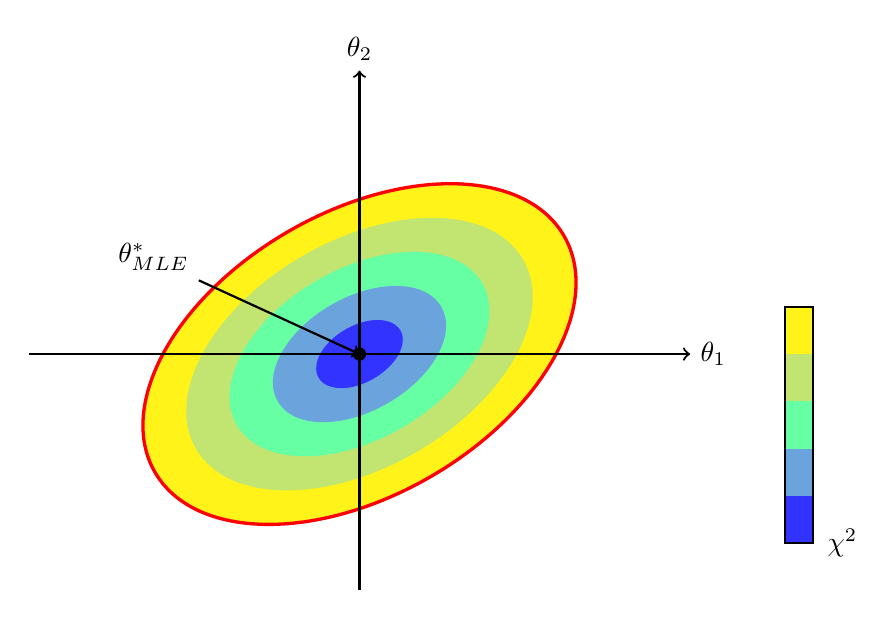
\begin{tikzpicture}[scale=1.2]
        \def\a{2.5}
        \def\b{1.5}
        \def\angle{30}
        
        \foreach \scale/\col in {1.0/yellow!90, 0.8/yellow!60!green!60, 0.6/green!60!cyan!60, 0.4/cyan!60!blue!60, 0.2/blue!80}{
            \fill[\col, rotate=\angle] (0,0) ellipse ({\a*\scale} and {\b*\scale});
        }
        
        % outer boundary (chi^2_max)
        \draw[red, very thick, rotate=\angle] (0,0) ellipse ({\a} and {\b});
        
        % axes
        \draw[->, thick] (-3.5,0) -- (3.5,0) node[right] {$\theta_1$};
        \draw[->, thick] (0,-2.5) -- (0,3) node[above] {$\theta_2$};
        
        % MLE point
        \fill (0,0) circle (2pt);
        \draw[<-, thick] (0,0) -- (-1.7,0.78) node[above left] {$\boldsymbol{\theta}^*_{\text{MLE}}$};
        
        % cbar
        \begin{scope}[shift={(4.5,0)}]
            \foreach \y/\col in {-2/blue!80, -1.5/cyan!60!blue!60, -1/green!60!cyan!60, -0.5/yellow!60!green!60, 0/yellow!90}{
                \fill[\col] (0,\y) rectangle (0.3,\y+0.5);
            }
            \draw[thick] (0,-2) rectangle (0.3,0.5);
            \node[right] at (0.35,-2) {$\chi^2$};
            \node[right] at (0.35,0.5) {};
        \end{scope}
    \end{tikzpicture}
    \caption{A hyperellipse confidence region in 2D, illustrating the region of indifference around the best-fit parameter estimate $\boldsymbol{\theta}^*_{\text{MLE}}$. The color scale indicates the $\chi^2$ value, with the red boundary marking $\chi^2(\boldsymbol{\theta}) = \chi^2_{\text{max}}$.}
    \label{fig:hyperellipse}
\end{figure}

The geometry of this ellipse tells us everything about our parameter uncertainties. If the matrix $\mathbf{V}_{\boldsymbol{\theta}}$ is diagonal, its inverse is also diagonal, and the ellipse's axes are aligned with the parameter axes (left panel of \autoref{fig:corr_uncorr}). This means there is no correlation between the uncertainties in our parameters; an error in estimating $\theta_1$ is independent of the error in estimating $\theta_2$. 

In general, $\mathbf{V}_{\boldsymbol{\theta}}$ is not diagonal. The off-diagonal terms represent the covariance between parameters, with the correlation coefficient between parameters $i$ and $j$ given by $\rho_{ij} = [\mathbf{V}_{\boldsymbol{\theta}}]_{ij}/(\sigma_{\theta_i}\sigma_{\theta_j})$. This results in a tilted ellipse that means that the parameter uncertainties are correlated (right panel of \autoref{fig:corr_uncorr}). The tilt shows that an overestimation of one parameter can be partially compensated for by an under- or overestimation of another. In other words, information about one parameter constrains the other. The overall volume of this uncertainty ellipse is proportional to $\sqrt{\det(\mathbf{V}_{\boldsymbol{\theta}})}$, which represents the total parameter uncertainty volume in $n$-dimensional space.

\begin{figure}[h!]
    \centering
    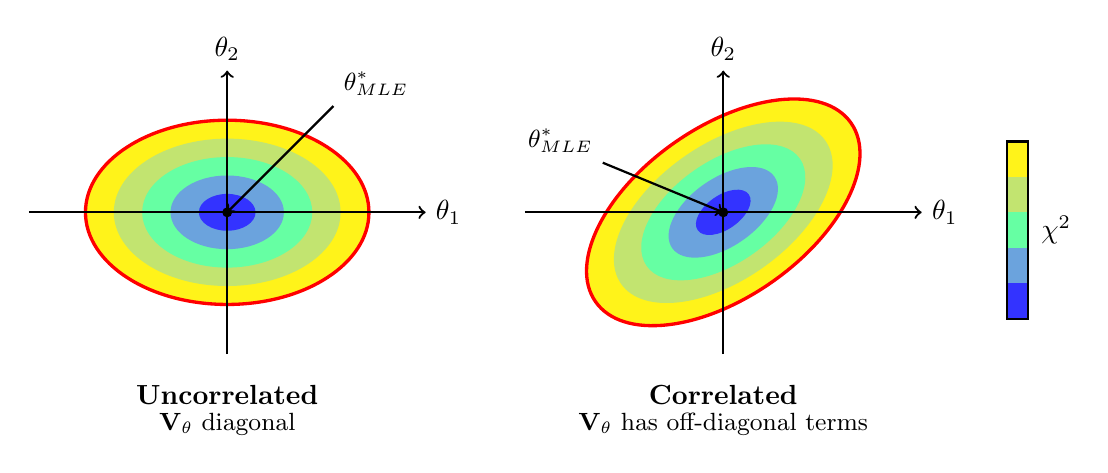
\begin{tikzpicture}[scale=0.9]
        \begin{scope}
            \def\a{2}
            \def\b{1.3}
            
            \foreach \scale/\col in {1.0/yellow!90, 0.8/yellow!60!green!60, 0.6/green!60!cyan!60, 0.4/cyan!60!blue!60, 0.2/blue!80}{
                \fill[\col] (0,0) ellipse ({\a*\scale} and {\b*\scale});
            }
            
            \draw[red, very thick] (0,0) ellipse ({\a} and {\b});
            
            \draw[->, thick] (-2.8,0) -- (2.8,0) node[right] {$\theta_1$};
            \draw[->, thick] (0,-2) -- (0,2) node[above] {$\theta_2$};
            
            \fill (0,0) circle (2pt);
            \draw[<-, thick] (0,0) -- (1.5,1.5) node[above right, font=\small] {$\boldsymbol{\theta}^*_{\text{MLE}}$};
            
            \node[below] at (0,-2.3) {\textbf{Uncorrelated}};
            \node[below, font=\small] at (0,-2.7) {$\mathbf{V}_{\boldsymbol{\theta}}$ diagonal};
        \end{scope}
        
        \begin{scope}[shift={(7,0)}]
            \def\a{2.2}
            \def\b{1.2}
            \def\angle{35}
            
            \foreach \scale/\col in {1.0/yellow!90, 0.8/yellow!60!green!60, 0.6/green!60!cyan!60, 0.4/cyan!60!blue!60, 0.2/blue!80}{
                \fill[\col, rotate=\angle] (0,0) ellipse ({\a*\scale} and {\b*\scale});
            }
            
            \draw[red, very thick, rotate=\angle] (0,0) ellipse ({\a} and {\b});
            
            \draw[->, thick] (-2.8,0) -- (2.8,0) node[right] {$\theta_1$};
            \draw[->, thick] (0,-2) -- (0,2) node[above] {$\theta_2$};
            
            \fill (0,0) circle (2pt);
            \draw[<-, thick] (0,0) -- (-1.7,0.7) node[above left, font=\small] {$\boldsymbol{\theta}^*_{\text{MLE}}$};
            
            \node[below] at (0,-2.3) {\textbf{Correlated}};
            \node[below, font=\small] at (0,-2.7) {$\mathbf{V}_{\boldsymbol{\theta}}$ has off-diagonal terms};
        \end{scope}
        
        \begin{scope}[shift={(11,0)}]
            \foreach \y/\col in {-1.5/blue!80, -1/cyan!60!blue!60, -0.5/green!60!cyan!60, 0/yellow!60!green!60, 0.5/yellow!90}{
                \fill[\col] (0,\y) rectangle (0.3,\y+0.5);
            }
            \draw[thick] (0,-1.5) rectangle (0.3,1);
            \node[right] at (0.35,1) {};
            \node[right] at (0.35,-0.25) {$\chi^2$};
        \end{scope}
    \end{tikzpicture}
    \caption{Left: An axis-aligned ellipse representing uncorrelated parameter uncertainties ($\mathbf{V}_{\boldsymbol{\theta}}$ is diagonal). Right: A tilted ellipse representing correlated parameter uncertainties ($\mathbf{V}_{\boldsymbol{\theta}}$ has off-diagonal elements). The red boundary in both cases marks $\chi^2(\boldsymbol{\theta}) = \chi^2_{\text{max}}$.}
    \label{fig:corr_uncorr}
\end{figure}

To better analyze these correlations, we can diagonalize the inverse covariance matrix, $\mathbf{V}_{\boldsymbol{\theta}}^{-1} = \mathbf{W}\mathbf{\Lambda}\mathbf{W}^\top$, where $\mathbf{\Lambda}$ is a diagonal matrix of eigenvalues $\lambda_i$ and $\mathbf{W}$ is the matrix of corresponding eigenvectors. The eigenvectors define the \textbf{principal axes} of the uncertainty ellipse, which are the directions in parameter space along which uncertainties are uncorrelated. By transforming our parameter deviations into this natural coordinate system, $\mathbf{q} = \mathbf{W}^\top \Delta\boldsymbol{\theta}$, the inequality simplifies beautifully to
\begin{equation}
    \sum_i \lambda_i q_i^2 \leq \chi^2_{\text{max}} - \chi^2(\boldsymbol{\theta}^*_{MLE})
\end{equation}
In this new basis, the parameter uncertainties are completely decoupled. The extent of the uncertainty region along each principal axis $q_i$ is easily found: $q_{i, \text{max}} = \sqrt{(\chi^2_{\text{max}} - \chi^2(\boldsymbol{\theta}^*_{MLE}))/\lambda_i}$. Smaller eigenvalues of $\mathbf{V}_{\boldsymbol{\theta}}^{-1}$ (equivalently, larger eigenvalues of $\mathbf{V}_{\boldsymbol{\theta}}$) correspond to larger uncertainties along that direction; that is, the data provides weaker constraints in those parameter combinations. This eigenvalue decomposition gives us a way to understand and report the principal uncertainties of our model fit.

\begin{figure}[h!]
    \centering
    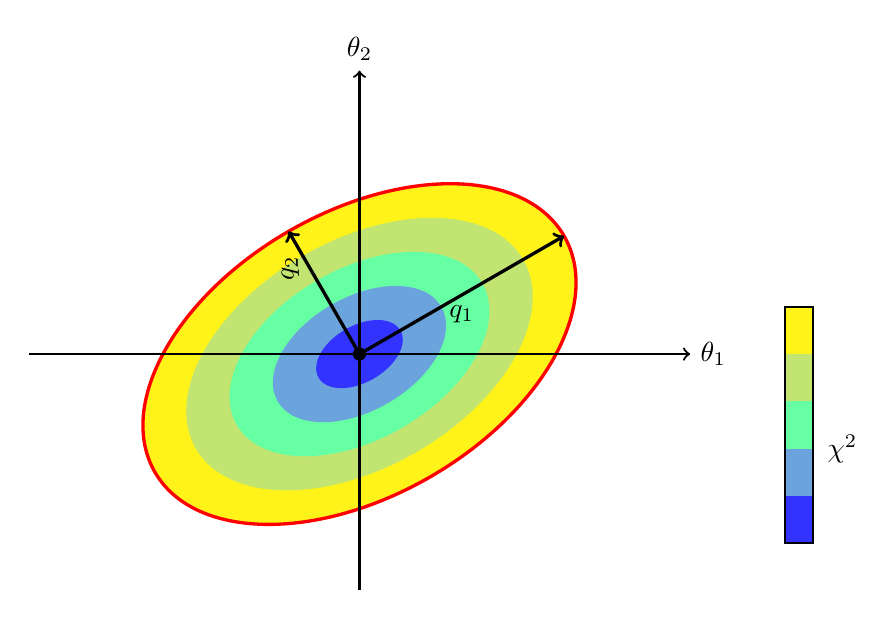
\begin{tikzpicture}[scale=1.2]
        \def\a{2.5}
        \def\b{1.5}
        \def\angle{30}
        
        \foreach \scale/\col in {1.0/yellow!90, 0.8/yellow!60!green!60, 0.6/green!60!cyan!60, 0.4/cyan!60!blue!60, 0.2/blue!80}{
            \fill[\col, rotate=\angle] (0,0) ellipse ({\a*\scale} and {\b*\scale});
        }
        
        % outer boundary
        \draw[red, very thick, rotate=\angle] (0,0) ellipse ({\a} and {\b});
        
        % original axes
        \draw[->, thick] (-3.5,0) -- (3.5,0) node[right] {$\theta_1$};
        \draw[->, thick] (0,-2.5) -- (0,3) node[above] {$\theta_2$};
        
        % principal axes
        \draw[->, very thick, rotate=\angle] (0,0) -- (\a,0) node[pos=0.5, below, sloped] {$q_1$};
        \draw[->, very thick, rotate=\angle] (0,0) -- (0,\b) node[pos=0.7, above, sloped] {$q_2$};
        
        % MLE point
        \fill (0,0) circle (2pt);
        % \draw[->, thick] (0,0) -- (1.2,0.8) node[midway, above right] {$\boldsymbol{\theta}^*_{\text{MLE}}$};
        
        % cbar
        \begin{scope}[shift={(4.5,0)}]
            \foreach \y/\col in {-2/blue!80, -1.5/cyan!60!blue!60, -1/green!60!cyan!60, -0.5/yellow!60!green!60, 0/yellow!90}{
                \fill[\col] (0,\y) rectangle (0.3,\y+0.5);
            }
            \draw[thick] (0,-2) rectangle (0.3,0.5);
            \node[right] at (0.35,-1) {$\chi^2$};
        \end{scope}
    \end{tikzpicture}
    \caption{The confidence ellipse shown with its principal axes $q_1$ and $q_2$, which are the eigenvectors of $\mathbf{V}_{\boldsymbol{\theta}}^{-1}$. In this rotated coordinate system, the parameter uncertainties are decoupled. The axis lengths are proportional to $1/\sqrt{\lambda_i}$, where $\lambda_i$ are the eigenvalues of $\mathbf{V}_{\boldsymbol{\theta}}^{-1}$ (or equivalently, proportional to $\sqrt{\lambda_i'}$ where $\lambda_i'$ are eigenvalues of $\mathbf{V}_{\boldsymbol{\theta}}$).}
    \label{fig:principal_axes}
\end{figure}

\begin{warningBox}
    \textbf{When the Ellipsoidal Approximation Breaks Down}
    
    The quadratic approximation underlying the ellipsoidal confidence regions is excellent for linear models and near the MLE for well-behaved nonlinear models. However, it can fail in several situations: (1) highly nonlinear models, (2) small sample sizes, and (3) parameter bounds or constraints. There exists other methods like profile likelihood methods to capture these cases, but we will not cover them here. They incur additional computational expense.
\end{warningBox}

\begin{warningBox}
    \textbf{Warning: Marginal Confidence Intervals and Parameter Correlations}
    
    \vspace{0.3cm}
    \begin{minipage}{0.55\textwidth}
        When parameters are correlated, reporting uncertainties as $\theta_i = \theta_i^* \pm \Delta\theta_i$ can be misleading. Consider the tilted confidence ellipse shown to the right. If we project this ellipse onto the $\theta_1$ axis, we obtain the interval $[a, b]$, which might tempt us to report
        \begin{equation*}
            \theta_1 = \theta_1^* \pm \frac{b-a}{2}
        \end{equation*}
        
        However, this interval is only valid when we allow $\theta_2$ to vary freely across all values consistent with the data. If we instead fix $\theta_2 = \theta_2^*$, the allowed range for $\theta_1$ is much smaller, as shown by the horizontal slice through the ellipse.
    \end{minipage}%
    \hfill
    \begin{minipage}{0.42\textwidth}
        \centering
        \begin{tikzpicture}[
            scale=.7,
            >=Stealth,
            every node/.style={font=\small},
            declare function={
              % helper trig (degrees)
              cs(\x)=cos(\x);
              ss(\x)=sin(\x);
            }
          ]
            % parameters
            \def\a{2.2}      % ellipse semi-axis along its local x
            \def\b{1.0}      % ellipse semi-axis along its local y
            \def\ang{-40}    % rotation in degrees
            \def\levels{{0.35,0.6,0.8,1.0}} % relative radii for nested contours (optional)
          
            % derived: correct half-widths on x
            \pgfmathsetmacro{\projhalf}{sqrt(\a*\a*cs(\ang)^2 + \b*\b*ss(\ang)^2)}
            \pgfmathsetmacro{\condhalf}{(\a*\b)/sqrt(\b*\b*cs(\ang)^2 + \a*\a*ss(\ang)^2)}
          
            % axes (draw FIRST so ellipse sits on top)
            \begin{scope}[line cap=round,line width=0.9pt]
              \draw[->] (-3.4,0) -- (3.6,0) node[below right=1pt] {$\theta_1$};
              \draw[->] (0,0) -- (0,2.6) node[above left=1pt] {$\theta_2$};
            \end{scope}
          
            % nested confidence levels (optional, for look of the 2nd pic)
            \foreach \r [count=\i] in \levels {
              \pgfmathsetmacro{\ra}{\r*\a}
              \pgfmathsetmacro{\rb}{\r*\b}
              \fill[rotate=\ang, fill opacity=0.2+0.15*\i, blue!40!green!20]
                   (0,0) ellipse ({\ra} and {\rb});
            }
          
            % outer ellipse boundary on top
            \draw[rotate=\ang, very thick, red] (0,0) ellipse ({\a} and {\b});
          
            % MLE point
            \fill (0,0) circle (2.4pt);
            \node[above right=1pt] at (0,0) {$\boldsymbol{\theta}^*_{\mathrm{MLE}}$};
          
            % conditional slice at theta2 = theta2* (y = 0)
            \draw[very thick, blue] (-\condhalf,0) -- (\condhalf,0);
            \node[blue] at (-\condhalf-0.25,+0.25) {$\theta_2=\theta_2^*$};

            % annotate conditional width (above line for clarity)
            % \draw[<->, thick, blue] (-\condhalf,0.45) -- (\condhalf,0.45)
            %       node[midway, above] {Conditional};

            % conditional projection line
            \draw[densely dashed, very thick, blue]
                  (-\condhalf,0) -- (-\condhalf,2.2);
            \draw[densely dashed, very thick, blue]
                  (\condhalf,0) -- (\condhalf,2.2);

          
            % marginal projection interval [a,b] on x
            % vertical guides at exact projection extrema
            \draw[densely dashed, very thick]
                  (-\projhalf,0) -- (-\projhalf,-2.2);
            \draw[densely dashed, very thick]
                  (\projhalf,0) -- (\projhalf,-2.2);

            % brace and label
            \draw[<->, thick] (-\projhalf,-1.6) -- (\projhalf,-1.6)
                  node[midway, below] {marginal: $[a,b]$};
          
            % ticks/labels a, theta1*, b on the axis like your 2nd image
            %\foreach \x/\lab in {-\projhalf/$a$,0/$\theta_1^*$,\projhalf/$b$}{
            %  \draw[black] (\x,0) -- (\x,-0.09) node[below=3pt] {\lab};
            %}
          
          \end{tikzpicture}
                  
    \end{minipage}
    
    \vspace{0.3cm}

    The marginal uncertainty (obtained by projection) is always larger than or equal to the conditional uncertainty (obtained by slicing at fixed values of other parameters). When reporting $\theta_1 = \theta_1^* \pm \sqrt{c_\alpha^2}\sigma_{\theta_1}$ as a confidence interval (or even just $\theta_1^* \pm \sigma_{\theta_1}$ as a standard error), we are implicitly reporting the marginal uncertainty. This marginal interval represents the range of $\theta_1$ values consistent with the data when $\theta_2$ is allowed to vary over all its plausible values. In contrast, if we \textit{knew} the true value of $\theta_2$ (which we don't), the uncertainty in $\theta_1$ would be smaller, as shown by the conditional slice. The full covariance matrix $\mathbf{V}_{\boldsymbol{\theta}}$ contains all the information about these correlations and should be reported alongside individual parameter uncertainties.
\end{warningBox}

\begin{exampleBox}
    \textbf{Example: Arrhenius Kinetics, Weighted Linear Regression, and Goodness-of-Fit} 
    
    In chemical kinetics, the Arrhenius model says that
    \begin{equation} 
        \ln k = \ln A - \dfrac{E_a}{R}\,\dfrac{1}{T}
    \end{equation}
    so with $x_i=1/T_i$ and $y_i=\ln k_i$, the model is linear: $y=\beta_0+\beta_1 x$ with $\beta_0=\ln A$ and $\beta_1=-E_a/R$. Using the heteroscedastic Gaussian errors $\sigma_i$ for $y_i=\ln k_i$, the WLS/MLE fit minimizes the same chi-square introduced above in \autoref{eq:chi-square-sum}, 
    \begin{equation}
        \chi^2(\beta_0,\beta_1)=\sum_{i=1}^{N}\frac{(y_i-\beta_0-\beta_1 x_i)^2}{\sigma_i^2}
    \end{equation}
    and returns $\hat{\boldsymbol\beta}=(\hat\beta_0,\hat\beta_1)$. For the ten temperatures shown in Fig.~\ref{fig:arrhenius-example}\subref{subfig:arrhenius-plot}, the optimum gives $\chi^2_{\mathrm{obs}}=7.58$, and with $n=2$ fitted parameters the degrees of freedom are 
    \begin{equation}
        \nu=N-n=8
    \end{equation}
    so the goodness-of-fit p-value is the upper tail
    \begin{equation}
        p = P\left(\chi^2_{\nu}\ge \chi^2_{\mathrm{obs}}\right) = P\left(\chi^2_{8}\ge 7.58\right)=0.476
    \end{equation}
    illustrated by the shaded survival area in Fig.~\ref{fig:arrhenius-example}\subref{subfig:chi2-tail}; the reduced statistic $\chi^2_\nu=\chi^2_{\mathrm{obs}}/\nu=0.95$ is close to the ``about one'' rule-of-thumb, so the linear Arrhenius model is not rejected. To quantify parameter uncertainty, we use \autoref{eq:parameter-covariance-matrix} to write the parameter covariance as
    \begin{equation}
        \mathbf{V}_{\boldsymbol\beta}=\left(\mathbf{J}^\top \mathbf{V}_\epsilon^{-1}\mathbf{J}\right)^{-1}
    \end{equation}
    so the marginal $95\%$ confidence intervals (likelihood-ratio view, $\Delta\chi^2=3.84$ for one parameter) are the familiar
    \begin{equation}
        \beta_0=\hat\beta_0\pm 1.96\sigma_{\beta_0}, \qquad 
        \beta_1=\hat\beta_1\pm 1.96\sigma_{\beta_1},
    \end{equation}
    which translate back to chemistry as $A=\exp(\beta_0)$ and $E_a=-R\beta_1$. Correlation between $\beta_0$ and $\beta_1$ is captured by the off-diagonal of $\mathbf{V}_{\boldsymbol\beta}$, and the \emph{joint} $95\%$ region is the ellipse
    \begin{equation}
        (\boldsymbol\beta-\hat{\boldsymbol\beta})^\top \mathbf{V}_{\boldsymbol\beta}^{-1}(\boldsymbol\beta-\hat{\boldsymbol\beta}) \le 5.99
    \end{equation}
    shown in Fig.~\ref{fig:arrhenius-example}\subref{subfig:beta-ellipse}. Hopefully it is clear how this example shows the flow of the theory above: (i) fit by minimizing $\chi^2$, (ii) judge absolute fit with the upper-tail p-value (survival function) at $\nu=N-n$, and (iii) read off marginal and joint parameter uncertainties from the Hessian geometry.

    \begin{figure}[H]
        \centering
        \begin{subfigure}[t]{0.32\textwidth}
          \centering
          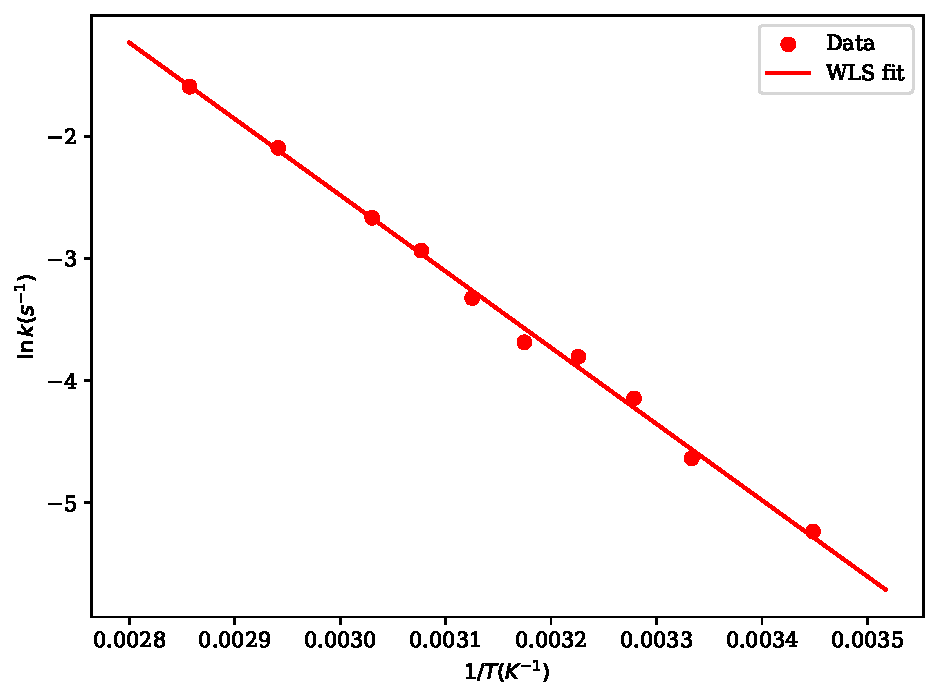
\includegraphics[width=\linewidth]{figs/models-vs-data/arrhenius_plot.pdf}
          \caption{Arrhenius plot: \(\ln k\) vs \(1/T\) with WLS line \(y=\hat\beta_0+\hat\beta_1 x\).}
          \label{subfig:arrhenius-plot}
        \end{subfigure}
        \hfill
        \begin{subfigure}[t]{0.32\textwidth}
          \centering
          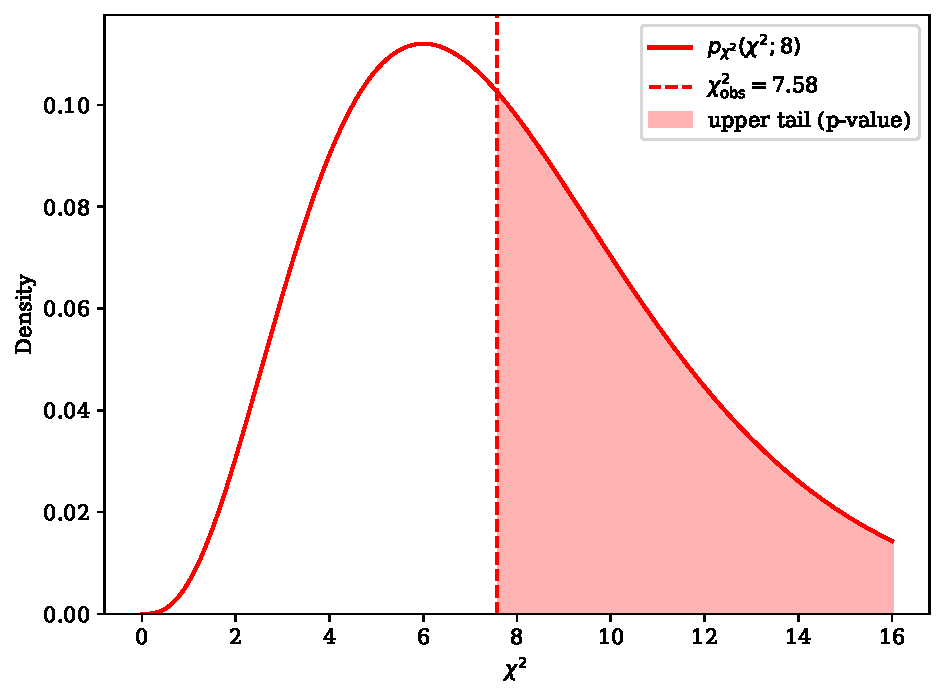
\includegraphics[width=\linewidth]{figs/models-vs-data/chi2_tail.pdf}
          \caption{Chi-square PDF for \(\nu=8\) with \(\chi^2_\text{obs}=7.58\) and shaded upper-tail p-value.}
          \label{subfig:chi2-tail}
        \end{subfigure}
        \hfill
        \begin{subfigure}[t]{0.32\textwidth}
          \centering
          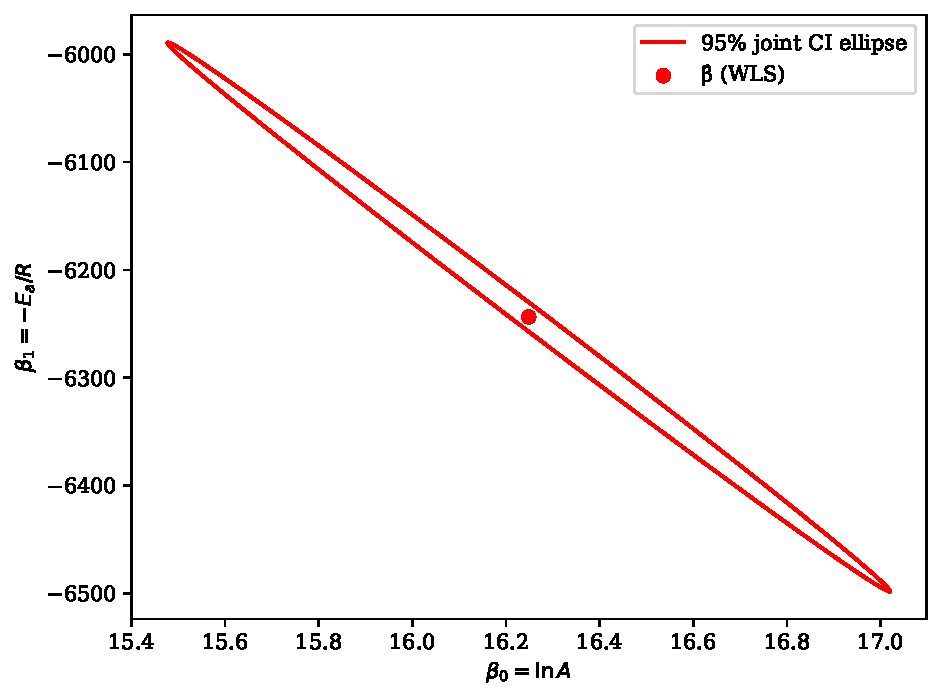
\includegraphics[width=\linewidth]{figs/models-vs-data/beta_joint_ellipse.pdf}
          \caption{Joint 95\% confidence ellipse in \((\beta_0,\beta_1)\)-space (\(\Delta\chi^2=5.99\)).}
          \label{subfig:beta-ellipse}
        \end{subfigure}
      
        \caption{Arrhenius WLS analysis: data and fit \subref{subfig:arrhenius-plot}, goodness-of-fit tail probability \subref{subfig:chi2-tail}, and joint parameter uncertainty \subref{subfig:beta-ellipse}.}
        \label{fig:arrhenius-example}
    \end{figure}
\end{exampleBox}

\section{The Bayesian View of Uncertainty}

The frequentist approach we have developed thus far treats the model parameters $\boldsymbol{\theta}$ as unknown but fixed quantities. We estimate them from the data, quantify their uncertainties through the parameter covariance matrix $\mathbf{V}_{\boldsymbol{\theta}}$, and construct confidence regions based on the chi-square distribution. This framework is powerful and widely used, but it represents only one philosophical perspective on the nature of uncertainty.

The Bayesian view offers a different interpretation. Rather than treating parameters as fixed unknowns, Bayesian inference regards the model parameters themselves as random variables that are described by a certain probability distribution. This perspective naturally incorporates our uncertainty about the parameters directly into the probabilistic framework. Before observing any data, we express our prior beliefs about the parameters through a prior distribution, $p(\boldsymbol{\theta})$. After observing data $\mathcal{D}$, we update these beliefs using Bayes' theorem to obtain the posterior distribution:
\begin{equation}
    p(\boldsymbol{\theta}|\mathcal{D}) = \frac{p(\mathcal{D}|\boldsymbol{\theta})p(\boldsymbol{\theta})}{p(\mathcal{D})} = \frac{p(\mathcal{D}|\boldsymbol{\theta})p(\boldsymbol{\theta})}{\int p(\mathcal{D}|\boldsymbol{\theta}')p(\boldsymbol{\theta}')d\boldsymbol{\theta}'}
\end{equation}
Here, $p(\mathcal{D}|\boldsymbol{\theta})$ is the likelihood function we encountered in the maximum likelihood framework, representing the probability of observing the data given a particular parameter value. The denominator, $p(\mathcal{D})$, is the evidence or marginal likelihood, which serves as a normalization constant ensuring that the posterior integrates to one. This normalization integral, which sums over all possible parameter values weighted by their prior probabilities and likelihoods, can be computationally challenging or even intractable, especially in high-dimensional parameter spaces.

The posterior distribution $p(\boldsymbol{\theta}|\mathcal{D})$ encapsulates all our updated knowledge about the parameters after seeing the data. Unlike the frequentist approach, which provides a single point estimate (the MLE) plus uncertainty quantification through confidence intervals, the Bayesian framework maintains the full probability distribution over parameter space. Uncertainty in the model parameters is naturally reflected by the shape and spread of this distribution. A narrow, concentrated posterior means that the data strongly constrains the parameters, while a broad posterior means significant remaining uncertainty even after observing the data.

To report parameter estimates in a format comparable to frequentist confidence intervals, Bayesian inference uses \textbf{credible intervals} (also called credible regions in higher dimensions). A credible interval $\Omega$ is defined such that the probability that the true parameter lies within this region, according to the posterior distribution, equals some specified value (typically 95\%):
\begin{equation}
    P(\boldsymbol{\theta} \in \Omega) = \int_{\Omega} p(\boldsymbol{\theta}|\mathcal{D})d\boldsymbol{\theta}
\end{equation}
The interpretation of a Bayesian credible interval is more intuitive than that of a frequentist confidence interval. A 95\% credible interval means there is a 95\% probability (given the data and our model assumptions) that the true parameter value lies within the interval. This is a direct probabilistic statement about the parameters themselves. In contrast, a frequentist 95\% confidence interval means that if we repeated the experiment many times and constructed intervals each time using the same procedure, 95\% of those intervals would contain the true parameter value---a more subtle distinction about the procedure rather than about this particular interval.

Any credible interval $\Omega$ can be used for this calculation, but conventionally we choose regions that contain the highest posterior density. Just as with the frequentist framework, we can also marginalize the joint posterior distribution to isolate the probability distribution for individual parameters. If $\boldsymbol{\theta} = (\theta_1, \theta_2, \ldots, \theta_n)$, the marginal posterior for parameter $\theta_i$ is obtained by integrating over all other parameters:
\begin{equation}
    p(\theta_i|\mathcal{D}) = \int p(\boldsymbol{\theta}|\mathcal{D})d\boldsymbol{\theta}_{\neq i}
\end{equation}
where $\boldsymbol{\theta}_{\neq i}$ denotes all parameters except $\theta_i$. This marginalization naturally accounts for correlations between parameters and provides the full distribution of our beliefs about each parameter individually, from which we can construct marginal credible intervals.

\section{\texorpdfstring{Conjugate Priors\textsuperscript{*}}{Conjugate Priors}}

While the Bayesian framework is conceptually elegant, a practical challenge immediately arises: how do we actually compute the posterior distribution? The normalization integral in the denominator of Bayes' theorem requires integrating the product of the likelihood and prior over the entire parameter space. For many combinations of likelihood functions and prior distributions, this integral has no closed-form analytical solution and must be evaluated numerically, often requiring computationally expensive Monte Carlo integration methods. Fortunately, there exists a special class of probability distributions called \textbf{exponential families} for which analytical solutions are possible when paired with appropriate priors. An exponential family is a probability distribution that can be written in the specific form:
\begin{equation}
    p_{\mathsf{x}}(x|\boldsymbol{\theta}) = h(x) \exp\left[\boldsymbol{\eta} \cdot \mathbf{T}(x) - A(\boldsymbol{\eta})\right]
\end{equation}
where $\boldsymbol{\eta}$ is the natural parameter vector (a function of $\boldsymbol{\theta}$), $\mathbf{T}(x)$ is the sufficient statistic, $h(x)$ is the base measure, and $A(\boldsymbol{\eta})$ is the log-partition function that ensures proper normalization. Many of the most commonly used probability distributions, including the normal (Gaussian), binomial, Poisson, exponential, gamma, and beta distributions, belong to exponential families.

For example, the normal distribution with mean $\mu$ and variance $\sigma^2$ can be written in exponential family form with natural parameters $\boldsymbol{\eta} = \left(\frac{\mu}{\sigma^2}, -\frac{1}{2\sigma^2}\right)$, sufficient statistics $\mathbf{T}(x) = (x, x^2)$, and
\begin{equation}
    h(x) = \frac{1}{\sqrt{2\pi}}, \qquad A(\boldsymbol{\eta}) = -\frac{\eta_1^2}{4\eta_2} - \frac{1}{2}\log(-2\eta_2)
\end{equation}
The key property of exponential families is that they possess \textbf{conjugate priors}, which are prior distributions that, when combined with the likelihood from the exponential family, give a posterior distribution in the same family as the prior. This closure property means that if the prior is in the conjugate family, the posterior can be computed in closed form simply by updating the parameters of that family. Conjugate priors make Bayesian inference analytically tractable and provide intuitive interpretations of how data updates our beliefs.

\begin{exampleBox}
    \textbf{Example: The Beta-Binomial Conjugacy}

    Consider the problem of evaluating whether a coin is fair by observing $N$ repeated tosses. The number of heads, $k$, follows a binomial distribution with unknown parameter $p$ (the true probability of heads):
    \begin{equation}
        p_{\mathsf{k}}(k; p) = \binom{N}{k}p^k(1-p)^{N-k}
    \end{equation}
    This is our likelihood function. To perform Bayesian inference, we need to specify a prior distribution for the unknown parameter $p$. Since $p$ must lie in the interval $[0,1]$ and we want a flexible distribution that can represent various prior beliefs, the natural choice is the beta distribution, which is the conjugate prior for the binomial likelihood:
    \begin{equation}
        p_{\mathsf{p}}(p; \alpha, \beta) = \frac{p^{\alpha-1}(1-p)^{\beta-1}}{B(\alpha,\beta)}
    \end{equation}
    The parameters $\alpha$ and $\beta$ control the shape of the prior. Setting $\alpha = \beta = 1$ yields a uniform prior (expressing complete ignorance), while larger values of $\alpha$ relative to $\beta$ express a prior belief that the coin is biased toward heads.

    After observing $N_H$ heads and $N_T$ tails (where $N = N_H + N_T$), we apply Bayes' theorem. The posterior is proportional to the product of the likelihood and prior:
    \begin{equation}
        p_{\mathsf{p}|\mathcal{D}}(p|N_H, N_T) \propto p^{N_H}(1-p)^{N_T} \times p^{\alpha-1}(1-p)^{\beta-1} \propto p^{\alpha+N_H-1}(1-p)^{\beta+N_T-1}
    \end{equation}
    Recognizing this functional form as another beta distribution, we can immediately write down the normalized posterior:
    \begin{equation}
        p_{\mathsf{p}|\mathcal{D}}(p|N_H, N_T) = \frac{p^{\alpha+N_H-1}(1-p)^{\beta+N_T-1}}{B(\alpha+N_H, \beta+N_T)}
    \end{equation}
    The posterior is a beta distribution with updated parameters $\alpha' = \alpha + N_H$ and $\beta' = \beta + N_T$. This elegant result shows that observing data simply adds the observed counts to the prior hyperparameters; the prior parameters $\alpha$ and $\beta$ can be interpreted as ``pseudo-counts'' representing our prior belief expressed as if we had already observed $\alpha-1$ heads and $\beta-1$ tails before the experiment began.

    Figure~\ref{fig:beta-binomial-conjugacy} illustrates several scenarios. When we start with a uniform prior ($\alpha = \beta = 1$) and observe balanced data ($N_H = N_T = 5$), the posterior is centered at $p = 0.5$ with moderate spread, reflecting the limited information from just ten tosses. With an informative prior ($\alpha = \beta = 5$) expressing a belief that the coin is fair, observing the same balanced data strengthens this belief, producing a narrower posterior. However, when we observe imbalanced data ($N_H = 8$, $N_T = 2$) with this same informative prior, we see the fundamental feature of Bayesian updating: the posterior represents a compromise between the prior belief and the evidence from the data. The likelihood alone would favor $p \approx 0.8$, but the prior pulls the posterior toward $p = 0.5$, resulting in a peak around $p \approx 0.65$.

    \begin{figure}[H]
        \centering
        \begin{subfigure}[t]{0.32\textwidth}
            \centering
            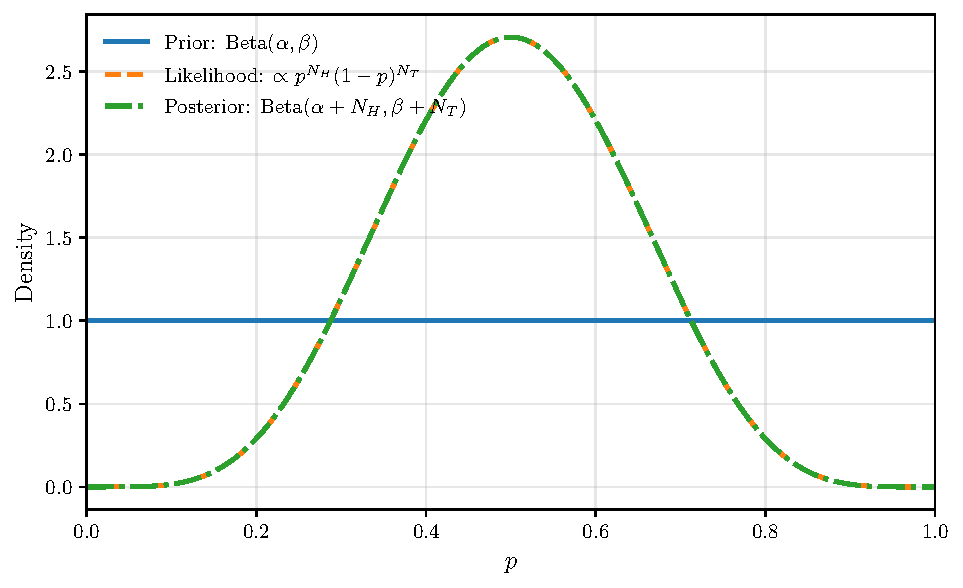
\includegraphics[width=\linewidth]{figs/models-vs-data/beta_binomial_uniform_balanced.pdf}
            \caption{Uniform prior; balanced data.}
            \label{fig:beta-binomial-uniform-balanced}
        \end{subfigure}\hfill
        \begin{subfigure}[t]{0.32\textwidth}
            \centering
            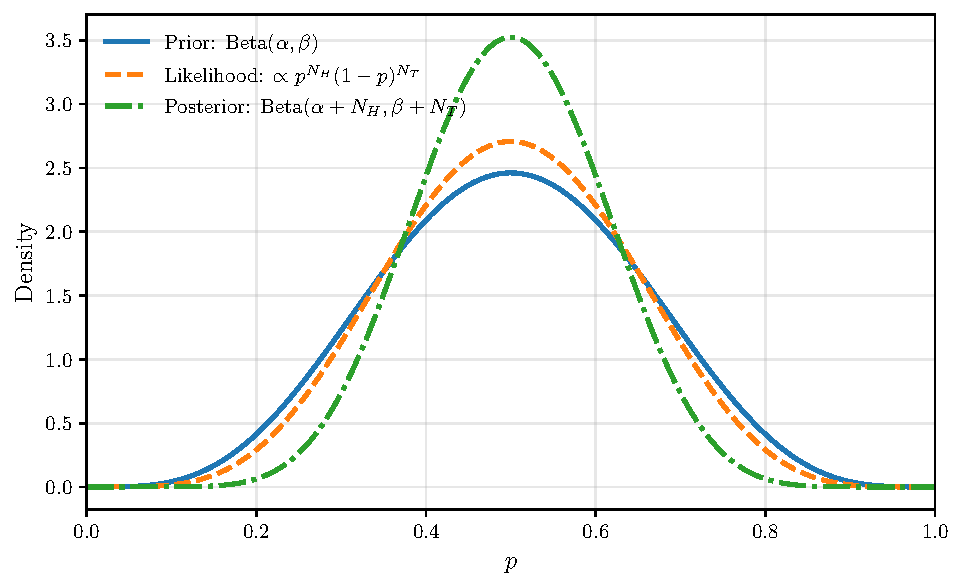
\includegraphics[width=\linewidth]{figs/models-vs-data/beta_binomial_informative_balanced.pdf}
            \caption{Informative symmetric prior; balanced data.}
            \label{fig:beta-binomial-informative-balanced}
        \end{subfigure}\hfill
        \begin{subfigure}[t]{0.32\textwidth}
            \centering
            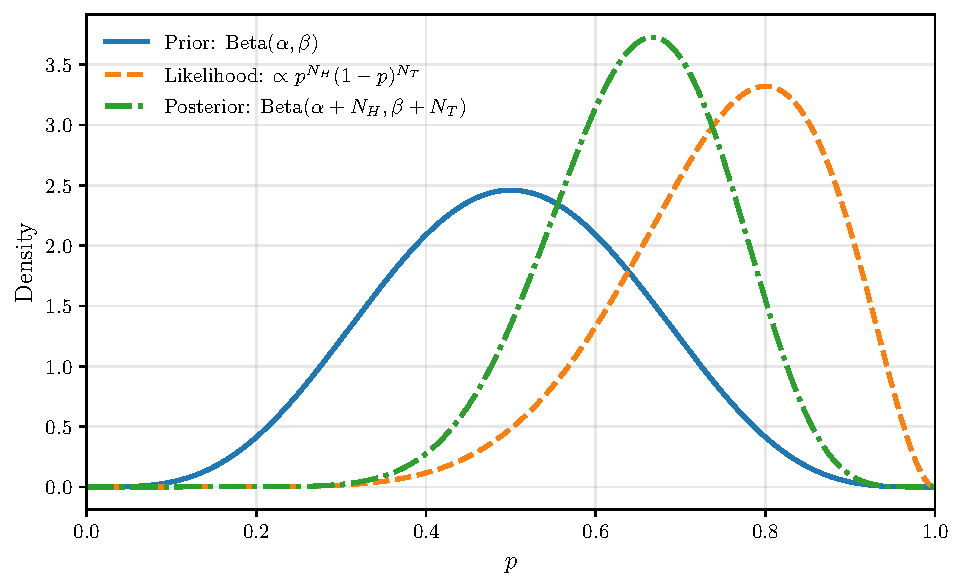
\includegraphics[width=\linewidth]{figs/models-vs-data/beta_binomial_informative_imbalanced.pdf}
            \caption{Informative symmetric prior; imbalanced data.}
            \label{fig:beta-binomial-informative-imbalanced}
        \end{subfigure}
        \caption{Bayesian inference for a coin flip experiment using beta--binomial conjugacy. Each panel shows the prior (blue), likelihood (orange), and posterior (yellow): (left) uniform prior with balanced data, (middle) informative symmetric prior with balanced data, (right) informative symmetric prior with imbalanced data showing how strong priors resist being updated by contradictory evidence.}
        \label{fig:beta-binomial-conjugacy}
    \end{figure}

    An even more striking illustration appears when we use a very strong prior ($\alpha = \beta = 50$), shown in Figure~\ref{fig:beta-binomial-strong-prior}. This prior encodes a strong belief that the coin is fair, equivalent to having already observed 98 prior tosses split evenly. Even when the actual data shows $N_H = 8$ and $N_T = 2$, suggesting bias, the posterior barely shifts from the prior. This demonstrates both the power and potential danger of strong priors: they allow us to incorporate genuine prior knowledge, but they also resist being updated by new evidence. The choice of prior is therefore not merely a technical detail but a substantive modeling decision that affects our conclusions.

    \begin{figure}[H]
        \centering
        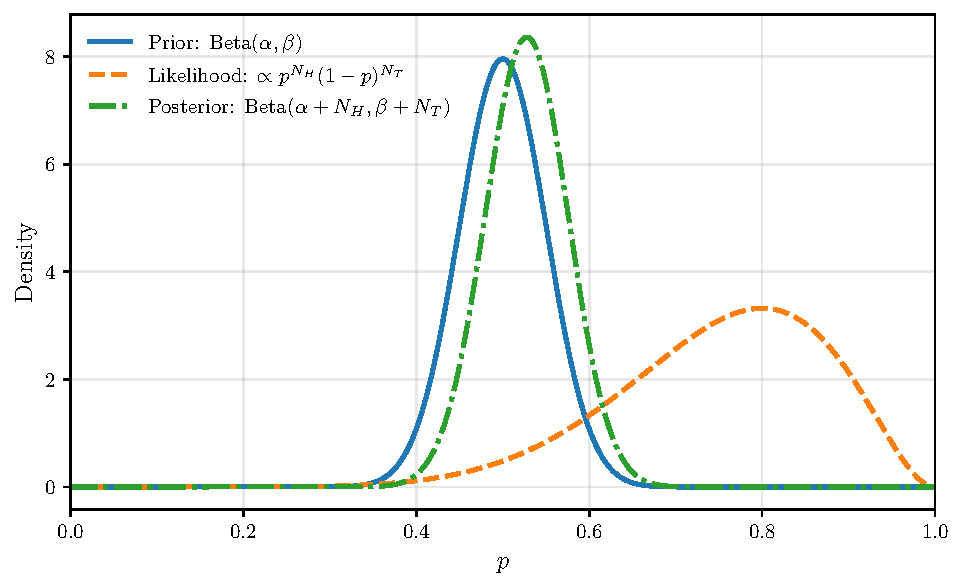
\includegraphics[width=0.4\textwidth]{figs/models-vs-data/beta_binomial_strong_prior.pdf}
        \caption{Effect of a strong prior ($\alpha = \beta = 50$) on Bayesian inference. Despite observing data ($N_H = 8$, $N_T = 2$) that suggests the coin is biased toward heads, the posterior (yellow) remains close to the prior (blue), demonstrating how strong prior beliefs resist updating even in the face of contradictory evidence.}
        \label{fig:beta-binomial-strong-prior}
    \end{figure}
\end{exampleBox}

Beyond the beta-binomial conjugacy, other important conjugate pairs exist throughout the exponential family. The normal distribution with known variance has a normal conjugate prior for its mean. The Poisson distribution has a gamma conjugate prior for its rate parameter. In general, exponential family distributions have conjugate priors that belong to a related exponential family, making them especially convenient for iterative Bayesian updating as more data arrives. When conjugate priors are not available or appropriate for the problem at hand, computational methods such as Markov chain Monte Carlo or variational inference must be employed to approximate the posterior distribution; we'll learn more about the former later!

\section{Prediction Uncertainty}

Both the frequentist and Bayesian frameworks provide methods for quantifying uncertainty in model parameters, but we are often interested in a related question: how uncertain are we about predictions made by the model at new, unobserved points? When we use our fitted model to predict an outcome $\tilde{y}$ at a new input location $\mathbf{x}$, the prediction itself is uncertain for two reasons. First, there is uncertainty in the parameters $\boldsymbol{\theta}$ used to make the prediction. Second, even if we knew the parameters perfectly, there is irreducible measurement noise $\boldsymbol{\epsilon}$ that would cause the observed value to differ from the model's deterministic prediction.

In the frequentist framework, we use the parameter covariance matrix $\mathbf{V}_{\boldsymbol{\theta}}$ to propagate parameter uncertainty into prediction uncertainty. For a linear model $\tilde{y}(\mathbf{x}; \boldsymbol{\theta}) = \mathbf{x}^\top\boldsymbol{\theta}$, the prediction $\tilde{y}$ is itself a linear function of the random variables $\boldsymbol{\theta}$. If the parameter estimates have mean $\boldsymbol{\theta}^*_{\text{MLE}}$ and covariance $\mathbf{V}_{\boldsymbol{\theta}}$, then the prediction has mean $\mu_{\tilde{y}} = \mathbf{x}^\top\boldsymbol{\theta}^*_{\text{MLE}}$ and variance
\begin{equation}
    \sigma^2_{\tilde{y}} = \mathbf{x}^\top \mathbf{V}_{\boldsymbol{\theta}} \mathbf{x}
\end{equation}
This variance quantifies only the contribution from parameter uncertainty. The total prediction uncertainty must also account for measurement noise. If the observations have error variance $\sigma^2_{\epsilon}$, the total variance of a new observation at $\mathbf{x}$ is
\begin{equation}
    \sigma^2_{\text{total}} = \sigma^2_{\tilde{y}} + \sigma^2_{\epsilon} = \mathbf{x}^\top \mathbf{V}_{\boldsymbol{\theta}} \mathbf{x} + \sigma^2_{\epsilon}
\end{equation}

For nonlinear models $\tilde{y}(\mathbf{x}; \boldsymbol{\theta})$, we cannot compute prediction uncertainty exactly, but we can use a first-order Taylor expansion around the MLE, just as we did for the confidence ellipse. The variance is approximately
\begin{equation}
    \sigma^2_{\tilde{y}} \approx \left.\frac{\partial \tilde{y}}{\partial \boldsymbol{\theta}}\right|_{\mathbf{x}}^\top \mathbf{V}_{\boldsymbol{\theta}} \left.\frac{\partial \tilde{y}}{\partial \boldsymbol{\theta}}\right|_{\mathbf{x}}
\end{equation}
where the gradient is evaluated at the MLE and at the prediction point $\mathbf{x}$. This linearization approach provides a local approximation to the prediction uncertainty and is widely used in practice.

\begin{exampleBox}
\textbf{Example: Prediction Uncertainty in a Temperature Model}

Consider a two-parameter model $\tilde{T}(r; \boldsymbol{\theta})$ that predicts temperature as a function of radius $r$, where $\boldsymbol{\theta} = (T_{\text{surf}}, \dot{q})$ represents the surface temperature and an internal heat generation parameter. Suppose the parameters have a diagonal covariance matrix (i.e., they are independent), so
\begin{equation}
    \mathbf{V}_{\boldsymbol{\theta}} = \begin{bmatrix} \sigma^2_{T_{\text{surf}}} & 0 \\ 0 & \sigma^2_{\dot{q}} \end{bmatrix}
\end{equation}
To predict the temperature at a new radius $r$ with uncertainty, we first compute the sensitivity of the model to each parameter:
\begin{equation}
    \sigma^2_{\tilde{T}}(r) = \left[\left.\frac{\partial \tilde{T}}{\partial T_{\text{surf}}}\right|_r, \left.\frac{\partial \tilde{T}}{\partial \dot{q}}\right|_r\right] \begin{bmatrix} \sigma^2_{T_{\text{surf}}} & 0 \\ 0 & \sigma^2_{\dot{q}} \end{bmatrix} \begin{bmatrix} \left.\frac{\partial \tilde{T}}{\partial T_{\text{surf}}}\right|_r \\ \left.\frac{\partial \tilde{T}}{\partial \dot{q}}\right|_r \end{bmatrix}
\end{equation}
Expanding this expression:
\begin{equation}
    \sigma_T(r) \sim \left[\left(\frac{\partial T(r)}{\partial T_{\text{surf}}} \sigma_{T_{\text{surf}}}\right)^2 + \left(\frac{\partial T(r)}{\partial \dot{q}} \sigma_{\dot{q}}\right)^2\right]^{1/2}
\end{equation}
This shows that the prediction uncertainty is a weighted combination of the individual parameter uncertainties, where the weights are the sensitivities of the prediction to each parameter. At locations where the model is highly sensitive to $T_{\text{surf}}$ (such as near the surface), uncertainty in that parameter dominates the prediction uncertainty. Conversely, at locations where the model is more sensitive to $\dot{q}$, uncertainty in the heat generation parameter becomes more important.
\end{exampleBox}

The Bayesian approach to prediction uncertainty is conceptually more comprehensive. Rather than propagating uncertainty from a point estimate through a linearization, Bayesian prediction explicitly acknowledges that we do not know the true parameter values and instead have a probability distribution $p(\boldsymbol{\theta}|\mathcal{D})$ representing our beliefs. When making a prediction at a new point $\mathbf{x}$, we should account for all plausible parameter values weighted by their posterior probabilities. The \textbf{posterior predictive distribution} is obtained by marginalizing over the parameter uncertainty:
\begin{equation}
    p(y|\mathbf{x}, \mathcal{D}) = \int p(y|\mathbf{x}, \boldsymbol{\theta}')p(\boldsymbol{\theta}'|\mathcal{D})d\boldsymbol{\theta}'
\end{equation}
Here, $p(y|\mathbf{x}, \boldsymbol{\theta}')$ is the likelihood at the new point, or the probability of observing outcome $y$ if the parameters were $\boldsymbol{\theta}'$, and $p(\boldsymbol{\theta}'|\mathcal{D})$ is the posterior distribution over parameters given the observed data. This integral effectively averages predictions across all possible parameter values, weighted by how probable each parameter value is given the data.

The posterior predictive distribution $p(y|\mathbf{x}, \mathcal{D})$ is the full probability distribution for the new observation, naturally incorporating both parameter uncertainty (through the integral over the posterior) and measurement noise (through the likelihood $p(y|\mathbf{x}, \boldsymbol{\theta}')$). From this distribution, we can extract point predictions (such as the mean or mode), prediction intervals, or any other quantity of interest. However, just as computing the posterior distribution required integrating the likelihood times the prior, computing the posterior predictive distribution requires another potentially difficult integral. When closed-form solutions are not available, Monte Carlo methods provide a practical computational approach: we draw samples $\boldsymbol{\theta}^{(1)}, \boldsymbol{\theta}^{(2)}, \ldots, \boldsymbol{\theta}^{(M)}$ from the posterior $p(\boldsymbol{\theta}|\mathcal{D})$, make a prediction with each sampled parameter set, and the distribution of these predictions approximates the posterior predictive distribution.

\section{Frequentist vs.\ Bayesian: A Summary}

We have now developed two parallel frameworks for quantifying uncertainty in models and their predictions. It is worth pausing to compare and contrast these approaches, as each has its own strengths, limitations, and appropriate contexts for application.

In the frequentist view, which we developed through maximum likelihood estimation and chi-square analysis, model parameters are treated as unknown but fixed quantities. We summarize the likelihood function using the chi-square statistic, assuming Gaussian measurement errors, to assess the significance of discrepancies between model and data. The chi-square distribution provides a formal hypothesis testing framework: we can identify regions of indifference in parameter space in which the chi-square goodness-of-fit test does not reject the model. These regions form confidence ellipsoids around the maximum likelihood estimate. The size and shape of these ellipsoids are determined by the local curvature of the chi-square surface, encoded in the parameter covariance matrix $\mathbf{V}_{\boldsymbol{\theta}} = (\mathbf{J}^\top\mathbf{V}_{\epsilon}^{-1}\mathbf{J})^{-1}$. For prediction uncertainty, we linearize the model at the MLE and propagate parameter uncertainties through the model's sensitivity derivatives, treating predictions as approximately normally distributed with variance $\mathbf{x}^\top\mathbf{V}_{\boldsymbol{\theta}}\mathbf{x}$ plus measurement noise.

The frequentist approach has several notable advantages. It requires minimal assumptions beyond the error model since we do not need to specify prior beliefs about parameters. The central limit theorem provides a theoretical justification for the asymptotic normality of parameter estimates and the validity of the chi-square distribution for large sample sizes, even when the underlying errors are not exactly Gaussian. The computations are typically straightforward: find the MLE through optimization, compute the Hessian (or its Gauss-Newton approximation), and invert to obtain the covariance matrix. The framework provides well-calibrated hypothesis tests with clear significance levels and p-values. However, the frequentist approach has limitations. The interpretation of confidence intervals is subtle: they describe the long-run frequency properties of the procedure rather than making probability statements about this particular interval containing the true parameter. The local quadratic approximation underlying the confidence ellipse can break down for highly nonlinear models or when far from the MLE. The method provides no natural way to incorporate external information or constraints beyond what is in the current dataset. Perhaps most importantly, once we have the MLE and covariance matrix, we discard information about the shape of the full likelihood surface, which may contain important asymmetries or multiple modes.

The Bayesian framework gives us a different view. Parameters are treated as random variables described by probability distributions. We begin with a prior distribution $p(\boldsymbol{\theta})$ encoding our beliefs before seeing data, then update to a posterior distribution $p(\boldsymbol{\theta}|\mathcal{D})$ using Bayes' theorem. The posterior distribution represents the complete state of our knowledge about the parameters after observing the data. We define credible intervals as regions where the probability (according to the posterior) that the true parameter lies within that region equals some specified value. The interpretation is direct and intuitive: a 95\% credible interval means there is a 95\% probability the parameter lies in that interval given the data and model. For predictions, we compute the posterior predictive distribution $p(y|\mathbf{x}, \mathcal{D})$ by marginalizing over parameter uncertainty, naturally accounting for our incomplete knowledge of the parameters.

The Bayesian framework's advantages include its intuitive probabilistic interpretation, its natural incorporation of prior information (from previous experiments, physical constraints, or expert knowledge), and its provision of the full posterior distribution rather than just a point estimate and covariance. It handles nonlinear models gracefully without relying on linearization approximations. Sequential updating is straightforward: today's posterior becomes tomorrow's prior when new data arrives. The framework provides a principled way to perform model comparison through Bayes factors or the evidence $p(\mathcal{D})$. Yet Bayesian inference also faces challenges. The choice of prior can be controversial or arbitrary, especially for problems where genuine prior information is lacking. The normalization integral in Bayes' theorem is often intractable, requiring sophisticated computational methods (MCMC, variational inference) that can be computationally expensive and slow to converge. Different priors can lead to different conclusions, particularly with limited data. The framework requires more assumptions (both the likelihood and the prior) and more computational machinery than frequentist approaches.

In practice, the two frameworks often produce similar results when data is abundant and informative. The frequentist confidence ellipse and the Bayesian credible region with a flat or weakly informative prior will often nearly coincide. The MLE and the MAP estimate converge as sample size increases and the prior becomes relatively less influential. However, the frameworks can diverge substantially in cases of limited data, strong prior information, or complex model structures. Many modern applications use hybrid approaches to get the computational efficiency of frequentist methods while still incorporating Bayesian ideas when prior information is valuable or when the full posterior distribution provides insights beyond point estimates.

\section{Optimal Experimental Design}

Before moving forward with more advanced modeling techniques, we should take a step back to think about why we run experiments in the first place. In some contexts, experiments serve a purely practical purpose. We might be physically manufacturing a molecule, synthesizing a new material, or producing a component where the experimental process itself is the end goal. However, more commonly in research settings, experiments are performed to obtain information. We run experiments to test hypotheses and assess whether data is consistent with theoretical predictions, to identify unknown parameters such as rate constants for reactive processes, to discriminate between competing candidate models that make different predictions, or to probe structure-function relationships in complex systems. Each of these objectives represents a different type of information-gathering task, and the experiments that are most valuable for one purpose may not be optimal for another.

This recognition leads naturally to the field of \textbf{optimal experimental design}, which provides formal frameworks for identifying the most informative or valuable experiments to perform given our objectives, constraints, and current state of knowledge. Rather than selecting experimental conditions arbitrarily or through trial and error, optimal design methods allow us to strategically choose where to sample, which variables to manipulate, and in what combinations in order to maximize the information gained per experiment. This is particularly important when experiments are expensive, time-consuming, dangerous, or limited by ethical considerations. The connection to our previous discussion of parameter uncertainty is very direct. As we saw before, identifying the maximum likelihood or maximum a posteriori estimate of parameters is a global optimization problem that may have many local minima, especially when we have a large number of parameters or when the model is highly nonlinear (such as those arising from ordinary differential equation initial value problem simulations). The choice of prior in Bayesian inference can lead to significant differences between MLE and MAP estimates. In both the frequentist and Bayesian views, we developed methods to quantify parametric uncertainty. Optimal experimental design takes these uncertainty quantification methods and inverts the question. Rather than asking how uncertain our parameters are given a particular dataset, we ask which experiments we should perform to minimize this uncertainty. 

\subsection{Space-Filling Designs}
When we do not have a trusted model structure, like when we lack confidence in assuming a simple linear relationship between inputs and outputs, a common approach is to use \textbf{space-filling designs}. These designs are agnostic to the specific model form and operate under the general premise that diversifying the inputs will lead to an informative distribution of outputs that can reveal the underlying system behavior. The philosophy is to spread experimental conditions throughout the input space so that whatever functional relationship exists between inputs and outputs, we will have sufficient coverage to detect it.

The simplest and perhaps most intuitive approach to experimentation is the \textbf{one-factor-at-a-time} (OFAT) strategy. In OFAT designs, we begin with a baseline set of conditions and then systematically vary each input factor individually while holding all others constant. For example, in a two-factor experiment with inputs $x_1$ and $x_2$, we might start at some central point and then create a series of experiments that explore variations in $x_1$ alone, followed by another series exploring $x_2$ alone (Figure~\ref{fig:ofat}). This approach has intuitive appeal and is straightforward to implement and interpret. However, OFAT designs have a major limitation: they cannot reliably estimate interaction effects between variables. Consider a model of the form $y = \theta_1 x_1 + \theta_2 x_2 + \theta_3 (x_1 x_2) + \epsilon$, where the output depends not only on the individual effects of $x_1$ and $x_2$ but also on their product. If we vary $x_1$ while holding $x_2$ fixed, the apparent effect of $x_1$ depends on which value of $x_2$ we chose to fix. By not exploring combinations where both factors vary simultaneously, OFAT misses the synergistic or antagonistic interactions that are often crucial to understanding system behavior.

\begin{figure}[H]
    \centering
    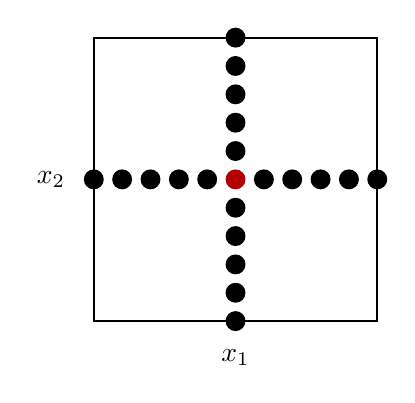
\begin{tikzpicture}[scale=1.2, every node/.style={scale=1}]
        \def\s{1.5}
        \def\n{4}
        
        \draw[thick] (-\s,-\s) rectangle (\s,\s);
        
        \node[below] at (0,-\s-0.2) {$x_1$};
        \node[left] at (-\s-0.2,0) {$x_2$};
        
        \fill[red!70!black] (0,0) circle (3pt);
        
        \foreach \i in {-4,-3,-2,-1,1,2,3,4}{
        \fill (0.3*\i,0) circle (3pt);
        }
    
        \foreach \i in {-4,-3,-2,-1,1,2,3,4}{
        \fill (0,0.3*\i) circle (3pt);
        }
    
        \fill (-\s,0) circle (3pt);
        \fill (\s,0) circle (3pt);
        \fill (0,-\s) circle (3pt);
        \fill (0,\s) circle (3pt);
    \end{tikzpicture}
    \caption{OFAT experimental design showing systematic variation of one factor at a time.}
    \label{fig:ofat}
\end{figure}

To address this limitation, \textbf{factorial designs} systematically explore combinations of input values. A \textbf{full factorial design} includes all possible combinations of input variables at a specified number of discrete levels. For instance, a $2^2$ factorial design for two factors at two levels each (typically denoted as low and high, or $-1$ and $+1$) consists of four experimental conditions corresponding to the corners of a square in the input space (Figure~\ref{fig:factorial2x2}). Similarly, a $5^2$ factorial design uses five levels for each of two factors, resulting in a grid of 25 experimental points (Figure~\ref{fig:factorial5x2}). Full factorial designs are comprehensive and allow for the estimation of all main effects and all interaction terms up to the highest order. However, the number of required experiments grows exponentially with the number of factors: a full factorial design for $N$ factors at two levels each requires $2^N$ experiments, which quickly becomes impractical for systems with many inputs. We note that with only two levels per factor, quadratic (curvature) terms (e.g., $x_i^2$) are not estimable without adding center or axial points (e.g., central composite designs) or using three or more levels per factor.

When the dimensionality is high and full factorial designs become prohibitively expensive, \textbf{fractional factorial designs} offer a practical compromise. These designs use a strategically chosen subset of the full factorial combinations, sacrificing the ability to estimate certain higher-order interactions in exchange for a dramatic reduction in the number of experiments. For example, a $2^{3-1}$ fractional factorial design uses only four experiments instead of the eight required for a full $2^3$ factorial (Figure~\ref{fig:fractional}). A common $2^{3-1}$ design might use the design matrix
\begin{equation}
    \mathbf{X} = \begin{bmatrix} -1 & -1 & 1 \\ 1 & -1 & -1 \\ -1 & 1 & -1 \\ 1 & 1 & 1 \end{bmatrix}
\end{equation}
representing the four vertices of a cube that are selected such that certain interaction effects are confounded (made indistinguishable) with main effects or with each other. The selection of which subset to use is guided by design theory that ensures main effects remain estimable while higher-order interactions (which are often less important) are aliased together. Fractional factorial designs are particularly valuable in screening experiments where the goal is to identify which of many potential factors significantly affect the output, with the understanding that more detailed exploration can follow.

\begin{figure}[H]
    \centering
    \begin{subfigure}[b]{0.3\textwidth}
        \centering
        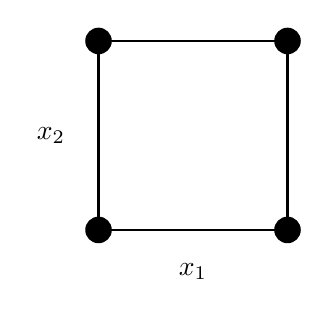
\begin{tikzpicture}[scale=1.2, every node/.style={scale=1}]
          \def\s{1.0}
        
          \draw[thick] (-\s,-\s) rectangle (\s,\s);
        
          \node[below] at (0,-\s-0.25) {$x_1$};
          \node[left] at (-\s-0.25,0) {$x_2$};
        
          \foreach \x in {-1,1}{
            \foreach \y in {-1,1}{
              \fill (\x*\s,\y*\s) circle (4pt);
            }
          }
        \end{tikzpicture}
        \caption{$2^2$ factorial design}
        \label{fig:factorial2x2}
    \end{subfigure}
    \hfill
    \begin{subfigure}[b]{0.3\textwidth}
        \centering
        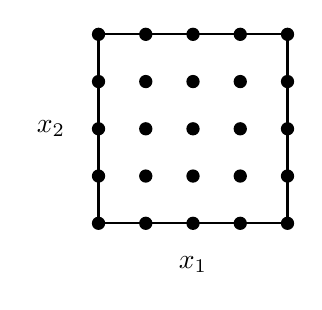
\begin{tikzpicture}[scale=1.2, every node/.style={scale=1}]
          \def\s{1.0}
        
          \draw[thick] (-\s,-\s) rectangle (\s,\s);
        
          \node[below] at (0,-\s-0.25) {$x_1$};
          \node[left] at (-\s-0.25,0) {$x_2$};
        
          \foreach \i in {-2,-1,0,1,2}{
            \foreach \j in {-2,-1,0,1,2}{
              \fill (0.5*\i,0.5*\j) circle (2pt);
            }
          }
        \end{tikzpicture}
        \caption{$5^2$ factorial design}
        \label{fig:factorial5x2}
    \end{subfigure}
    \hfill
    \begin{subfigure}[b]{0.3\textwidth}
        \centering
        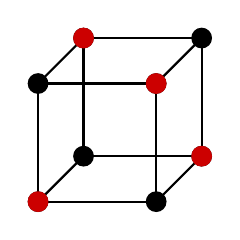
\begin{tikzpicture}[scale=1.5,line join=round,line cap=round,thick]
            \coordinate (A) at (0,0,0);
            \coordinate (B) at (1,0,0);
            \coordinate (C) at (1,1,0);
            \coordinate (D) at (0,1,0);
            \coordinate (E) at (0,0,1);
            \coordinate (F) at (1,0,1);
            \coordinate (G) at (1,1,1);
            \coordinate (H) at (0,1,1);
            
            \draw (A)--(B)--(C)--(D)--cycle;
            \draw (E)--(F)--(G)--(H)--cycle;
            \draw (A)--(E);
            \draw (B)--(F);
            \draw (C)--(G);
            \draw (D)--(H);
            
            \foreach \p in {A,B,C,D,E,F,G,H}{
              \fill[black] (\p) circle (2.5pt);
            }
            
            \foreach \p in {E,B,D,G}{
              \fill[red!80!black] (\p) circle (2.5pt);
            }
        \end{tikzpicture}
        \caption{$2^{3-1}$ fractional factorial}
        \label{fig:fractional}
    \end{subfigure}
    \caption{Factorial design configurations showing (a) full factorial with two factors at two levels, (b) full factorial with two factors at five levels, and (c) fractional factorial design highlighting a strategically chosen subset (red) of the full $2^3$ factorial (black).}
    \label{fig:factorial_designs}
\end{figure}

Beyond factorial designs, other space-filling approaches offer different advantages. \textbf{Box-Behnken designs} are subsets of $3^N$ factorial designs specifically constructed for fitting quadratic models (those including squared terms like $x_i^2$ in addition to linear and interaction terms). These designs place experimental points at the midpoints of edges and at the center of the design space, avoiding the corners (Figure~\ref{fig:boxbehnken}). They can include repeated measurements at the center point. These repeated points allow for assessment of pure experimental error, which can then be distinguished from lack-of-fit when the model is inadequate.

\begin{figure}[H]
    \centering
    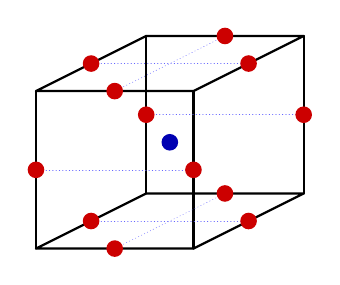
\begin{tikzpicture}[
        line join=round, line cap=round, thick,
        x={(-0.7cm,-0.35cm)}, y={(1.0cm,0cm)}, z={(0cm,1.0cm)},
        bbpoint/.style={circle,inner sep=0pt,minimum size=7pt},
        guide/.style={blue!60, very thin, densely dotted}
      ]
      
      % cube (from (-1,-1,-1) to (1,1,1))
      \draw (-1,-1,-1) -- ( 1,-1,-1) -- ( 1, 1,-1) -- (-1, 1,-1) -- cycle; % bottom
      \draw (-1,-1, 1) -- ( 1,-1, 1) -- ( 1, 1, 1) -- (-1, 1, 1) -- cycle; % top
      \draw (-1,-1,-1) -- (-1,-1, 1);
      \draw ( 1,-1,-1) -- ( 1,-1, 1);
      \draw ( 1, 1,-1) -- ( 1, 1, 1);
      \draw (-1, 1,-1) -- (-1, 1, 1);
      
      % zero-plane guide lines
      \draw[guide] (-1,0,-1) -- ( 1,0,-1);
      \draw[guide] (-1,0, 1) -- ( 1,0, 1);
      \draw[guide] (0,-1,-1) -- (0, 1,-1);
      \draw[guide] (0,-1, 1) -- (0, 1, 1);
      \draw[guide] (-1,-1,0) -- (-1, 1,0);
      \draw[guide] ( 1,-1,0) -- ( 1, 1,0);
      
      % Box–Behnken points: edge midpoints (red)
      \foreach \P in {(-1,-1,0), (-1, 1,0), ( 1,-1,0), ( 1, 1,0),
                      (-1,0,-1), (-1,0, 1), ( 1,0,-1), ( 1,0, 1),
                      (0,-1,-1), (0,-1, 1), (0, 1,-1), (0, 1, 1)}{
        \fill[red!80!black] \P circle (3pt);
      }
      
      % center point (blue)
      \fill[blue!70!black] (0,0,0) circle (3pt);
      
    \end{tikzpicture}
    \caption{Box-Behnken design showing edge midpoints (red) and center point (blue) for a three-factor experiment.}
    \label{fig:boxbehnken}
\end{figure}

\textbf{Latin hypercube designs} take a different approach and ensure that the marginal distribution of each input variable is uniform. Imagine dividing the range of each input into equally spaced intervals; a Latin hypercube design selects points such that each interval is sampled exactly once for each variable (Figure~\ref{fig:latinhypercube}). This creates excellent space-filling properties while using relatively few points. The name derives from the mathematical concept of a Latin square extended to higher dimensions. Latin hypercube sampling is popular in computer experiments and uncertainty quantification where we can evaluate the model cheaply and want to explore a high-dimensional input space efficiently.

\begin{figure}[H]
    \centering
    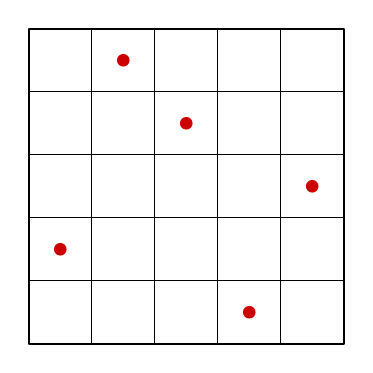
\begin{tikzpicture}[scale=4, line cap=round, line join=round]
        % parameters
        \def\n{5} % number of levels per axis
      
        % frame and grid
        \draw[thick] (0,0) rectangle (1,1);
        \foreach \i in {1,...,\numexpr\n-1\relax} {
          \draw (0,\i/\n) -- (1,\i/\n);   % horizontal
          \draw (\i/\n,0) -- (\i/\n,1);   % vertical
        }
      
        % Latin hypercube points
        \foreach \r/\c in {1/4, 2/1, 3/5, 4/3, 5/2} {
          \fill[red!80!black] ({(\c-0.5)/\n},{(\r-0.5)/\n}) circle (0.02);
        }
    \end{tikzpicture}
    \caption{Latin hypercube design with five levels per factor, ensuring each row and column contains exactly one sample point.}
    \label{fig:latinhypercube}
\end{figure}

\subsection{Model-Based Experimental Design for Linear Models}

While space-filling designs are valuable when we lack a trusted model, a more powerful approach becomes available when we do have a model structure in mind and want to design experiments specifically to estimate its parameters as accurately as possible. For linear models, we can develop this approach very cleanly. Recall from earlier that the parameter covariance matrix quantifying uncertainty in our estimated parameters is given by
\begin{equation}
    \mathbf{V}_{\boldsymbol{\theta}} = \left(\mathbf{J}^\top \mathbf{V}_{\boldsymbol{\epsilon}}^{-1} \mathbf{J}\right)^{-1}
\end{equation}
where $\mathbf{J}$ is the Jacobian matrix (or sensitivity matrix) with elements $J_{ij} = \partial \tilde{y}_i / \partial \theta_j$ describing how each model prediction depends on each parameter. If we assume that measurements are independent with equal variances, so that $\mathbf{V}_{\boldsymbol{\epsilon}} = \sigma^2 \mathbf{I}$, then for a linear model of the form $\tilde{y}(\mathbf{x}; \boldsymbol{\theta}) = \mathbf{X}\boldsymbol{\theta}$, the Jacobian is simply the design matrix itself: $\mathbf{J} = \mathbf{X}$. Therefore, the parameter covariance becomes
\begin{equation}
    \mathbf{V}_{\boldsymbol{\theta}} = \sigma^2 \left(\mathbf{X}^\top \mathbf{X}\right)^{-1}
    \label{eq:param-cov-design}
\end{equation}
So, in this case, the parametric uncertainty does not depend on the actual outcomes of the experiments, only on the input conditions we choose to explore! Before running any experiments, before collecting any data, we can predict exactly how uncertain our parameter estimates will be based solely on our choice of design matrix $\mathbf{X}$. This property enables us to optimize the experimental design in advance.

The matrix $\mathbf{X}^\top \mathbf{X}$ is known as the \textbf{Fisher information matrix}. It quantifies how much information about the parameters is contained in the chosen experimental design. A larger Fisher information matrix (in an appropriate matrix sense) corresponds to smaller parameter uncertainties. For nonlinear models, the sensitivity matrix $\mathbf{J}$ does depend on the parameter values, so we must evaluate it at some approximate parameter values $\boldsymbol{\theta} \approx \boldsymbol{\theta}^*_{\text{MLE}}$, perhaps from a pilot experiment or from prior knowledge. This introduces an iterative aspect to optimal design for nonlinear systems: we design experiments based on current parameter estimates, run those experiments to update the estimates, then redesign subsequent experiments based on the improved estimates.

To understand the importance of the Fisher information matrix, let's consider a simple example. Suppose we wish to fit a linear model with three parameters: $y = \theta_1 + \theta_2 x_1 + \theta_3 x_2 + \epsilon$. First of all, to see how this scalar equation translates to matrix form, consider a single experiment where we set the inputs to $x_1 = 2$ and $x_2 = 2$. For this experiment, the model becomes:
\begin{equation}
    y = \theta_1 \cdot 1 + \theta_2 \cdot 2 + \theta_3 \cdot 2 + \epsilon = [1, 2, 2][\theta_1, \theta_2, \theta_3]^\top + \epsilon
\end{equation}
If we run $n$ experiments with different input values $(x_1^{(i)}, x_2^{(i)})$ for $i = 1, \ldots, n$, stacking these rows gives the full matrix system:
\begin{equation}
    \begin{bmatrix} y^{(1)} \\ y^{(2)} \\ \vdots \\ y^{(n)} \end{bmatrix} = \begin{bmatrix} 1 & x_1^{(1)} & x_2^{(1)} \\ 1 & x_1^{(2)} & x_2^{(2)} \\ \vdots & \vdots & \vdots \\ 1 & x_1^{(n)} & x_2^{(n)} \end{bmatrix} \begin{bmatrix} \theta_1 \\ \theta_2 \\ \theta_3 \end{bmatrix} + \begin{bmatrix} \epsilon^{(1)} \\ \epsilon^{(2)} \\ \vdots \\ \epsilon^{(n)} \end{bmatrix}
\end{equation}
The matrix in the middle is our design matrix $\mathbf{X}$. Now, imagine we unwisely choose to run four experiments where the two input variables always take the same value: experiment 1 with $(x_1, x_2) = (1, 1)$, experiment 2 with $(2, 2)$, experiment 3 with $(3, 3)$, and experiment 4 with $(4, 4)$. This gives the design matrix:
\begin{equation}
    \mathbf{X} = \begin{bmatrix} 1 & 1 & 1 \\ 1 & 2 & 2 \\ 1 & 3 & 3 \\ 1 & 4 & 4 \end{bmatrix}
\end{equation}
Computing the Fisher information matrix, we get
\begin{equation}
    \mathbf{X}^\top \mathbf{X} = \begin{bmatrix} 4 & 10 & 10 \\ 10 & 30 & 30 \\ 10 & 30 & 30 \end{bmatrix}
\end{equation}
This matrix is singular. Conceptually, this occurs because we have no experiments where $x_1 \neq x_2$, so we cannot distinguish the effect of $\theta_2$ from that of $\theta_3$. The model is fundamentally unidentifiable with this design. Mathematically, the least squares solution $\boldsymbol{\theta}^* = (\mathbf{X}^\top \mathbf{X})^{-1} \mathbf{X}^\top \mathbf{y}$ requires inverting $\mathbf{X}^\top \mathbf{X}$, which is impossible when the matrix is singular. This is an extreme example of poor experimental design.

Even when we avoid complete singularity, poor designs can still lead to enormous parameter uncertainties. Consider a slight modification where we allow $x_1$ and $x_2$ to differ very slightly: experiments at $(x_1, x_2) = (1, 1)$, $(2, 2.01)$, $(3, 3.01)$, and $(4, 4.01)$:
\begin{equation}
    \mathbf{X} = \begin{bmatrix} 1 & 1 & 1 \\ 1 & 2 & 2.01 \\ 1 & 3 & 3.01 \\ 1 & 4 & 4.01 \end{bmatrix}
\end{equation}
Now the Fisher information matrix is technically invertible with
\begin{equation}
    \mathbf{X}^\top \mathbf{X} = \begin{bmatrix} 4 & 10 & 10.03 \\ 10 & 30 & 30.09 \\ 10.03 & 30.09 & 30.1803 \end{bmatrix}
\end{equation}
but its inverse reveals severe problems:
\begin{equation}
    \mathbf{V}_{\boldsymbol{\theta}} \propto \left(\mathbf{X}^\top \mathbf{X}\right)^{-1} \approx \begin{bmatrix} 1.5 & -0.5 & 6 \times 10^{-12} \\ -0.5 & 33534 & -33433 \\ 8 \times 10^{-12} & -33433 & 33333 \end{bmatrix}
\end{equation}
The diagonal elements, which represent the variances of individual parameters, are enormous for $\theta_2$ and $\theta_3$ (uncertainties on the order of $\sqrt{33534} \sigma \approx 183\sigma$). Moreover, the off-diagonal terms tell us that there is extreme correlation between these parameters. Because we are still choosing experiments where $x_1$ and $x_2$ barely vary relative to each other, the data cannot reliably separate their individual effects. Near-singularity is nearly as problematic as exact singularity.

In contrast, consider a better design where the input variables vary independently. Using just three experiments at $(x_1, x_2) = (1, 1)$, $(0, 1)$, and $(1, 0)$, we get the design matrix
\begin{equation}
    \mathbf{X} = \begin{bmatrix} 1 & 1 & 1 \\ 1 & 0 & 1 \\ 1 & 1 & 0 \end{bmatrix}
\end{equation}
with parameter covariance
\begin{equation}
    \mathbf{V}_{\boldsymbol{\theta}} = \sigma^2 \left(\mathbf{X}^\top \mathbf{X}\right)^{-1} = \begin{bmatrix} 3 & -2 & -2 \\ -2 & 2 & 1 \\ -2 & 1 & 2 \end{bmatrix} \sigma^2
\end{equation}
While there are still correlations (off-diagonal terms), the parameter variances (diagonal elements) are now on the order of $\sigma^2$ rather than tens of thousands of $\sigma^2$. This is a great improvement.

Let's now consider replication. If we repeat each of the three experiments in the design above, stacking them to create a larger design matrix, we get
\begin{equation}
    \mathbf{X}' = \begin{bmatrix} \mathbf{X}_1 \\ \mathbf{X}_2 \\ \vdots \\ \mathbf{X}_N \end{bmatrix} = \begin{bmatrix} 1 & 1 & 1 \\ 1 & 0 & 1 \\ 1 & 1 & 0 \\ \vdots & \vdots & \vdots \\ 1 & 1 & 1 \\ 1 & 0 & 1 \\ 1 & 1 & 0 \end{bmatrix}
\end{equation}
the parameter covariance becomes
\begin{equation}
    \mathbf{V}_{\boldsymbol{\theta}} = \sigma^2 \left(\mathbf{X}'^\top \mathbf{X}'\right)^{-1} = \frac{1}{N} \begin{bmatrix} 3 & -2 & -2 \\ -2 & 2 & 1 \\ -2 & 1 & 2 \end{bmatrix} \sigma^2
\end{equation}
where $N$ is the number of replications. The parameter uncertainties scale as $1/\sqrt{N}$, following the familiar statistical principle that uncertainty decreases with the square root of sample size. Statistical replication (performing the same experiment multiple times) therefore helps identify sources of true systematic variation in the output without obfuscation by measurement noise. Replicates do not provide new information about different parts of the input space, but they do improve our confidence in the parameter estimates by averaging out random errors.

\subsection{Optimality Criteria for Experimental Design}

We have established that for linear models with uncorrelated, homoscedastic errors, the parameter covariance matrix $\mathbf{V}_{\boldsymbol{\theta}} = \sigma^2 (\mathbf{X}^\top \mathbf{X})^{-1}$ quantifies the uncertainty in our parameter estimates as a function of the experimental design $\mathbf{X}$. But how do we choose the best design? The challenge is that $\mathbf{V}_{\boldsymbol{\theta}}$ is a matrix, not a scalar. We need to define what we mean by minimizing a matrix. Different objectives lead to different optimality criteria, each with its own interpretation and mathematical properties.

One natural approach is \textbf{A-optimality} (the ``A'' stands for ``average''), which minimizes the trace of the covariance matrix:
\begin{equation}
    \text{A-optimal:} \quad \min_{\mathbf{X}} \text{trace}(\mathbf{V}_{\boldsymbol{\theta}}) = \min_{\mathbf{X}} \sum_{i=1}^{n} [\mathbf{V}_{\boldsymbol{\theta}}]_{ii}
\end{equation}
The trace is the sum of the diagonal elements, which are the individual parameter variances. A-optimal designs therefore minimize the total variance of all parameters. They treat each parameter's uncertainty as equally important and ignore any correlations between parameters. This criterion is intuitive and computationally straightforward, so it is a popular choice in practice.

Perhaps the most widely used criterion is \textbf{D-optimality} (where ``D'' refers to ``determinant''), which minimizes the determinant of the covariance matrix:
\begin{equation}
    \text{D-optimal:} \quad \min_{\mathbf{X}} \det(\mathbf{V}_{\boldsymbol{\theta}}) = \min_{\mathbf{X}} \det\left[\left(\mathbf{X}^\top \mathbf{X}\right)^{-1}\right] \equiv \max_{\mathbf{X}} \det\left(\mathbf{X}^\top \mathbf{X}\right)
\end{equation}
The determinant of a matrix has a geometric interpretation as the volume of the parallelepiped defined by the matrix rows (or columns). In the context of parameter estimation, like we saw, $\det(\mathbf{V}_{\boldsymbol{\theta}})$ is proportional to the hypervolume of the confidence ellipsoid in parameter space. Minimizing this volume means making the region of indifference as small as possible, thereby constraining the parameters most tightly. D-optimal designs have nice theoretical properties and are equivalent to maximizing the determinant of the Fisher information matrix $\det(\mathbf{X}^\top \mathbf{X})$, which explains why D-optimality is often described as maximizing the information content of the design.

To illustrate the impact of design choices on D-optimality, let's reconsider the $2^{3-1}$ fractional factorial design with design matrix
\begin{equation}
    \mathbf{X} = \begin{bmatrix} -1 & -1 & 1 \\ 1 & -1 & -1 \\ -1 & 1 & -1 \\ 1 & 1 & 1 \end{bmatrix}
\end{equation}
For this design, $\det(\mathbf{X}^\top \mathbf{X}) = 64$, so if $\sigma^2 = 1$, then $\det(\mathbf{V}_{\boldsymbol{\theta}}) = 1/64$. Suppose we modify a single entry, changing the first element of the first column from $-1$ to $+1$:
\begin{equation}
    \mathbf{X} = \begin{bmatrix} +1 & -1 & 1 \\ 1 & -1 & -1 \\ -1 & 1 & -1 \\ 1 & 1 & 1 \end{bmatrix}
\end{equation}
This seemingly small change halves the determinant: $\det(\mathbf{X}^\top \mathbf{X}) = 32$, corresponding to $\det(\mathbf{V}_{\boldsymbol{\theta}}) = 1/32$. The confidence ellipsoid volume has doubled; the design is now significantly worse. Had we instead used the full $2^3$ factorial design with eight experiments, we would achieve $\det(\mathbf{X}^\top \mathbf{X}) = 512$ (so $\det(\mathbf{V}_{\boldsymbol{\theta}}) = 1/512$). The full design provides eight times smaller ellipsoid volume (in the D-optimal sense) compared to the half-fraction, which is sensible given that it uses twice as many experiments.

\begin{figure}[h!]
    \centering
    \captionsetup[sub]{justification=centering}
    
    % --------- reusable cube macro ----------
    % Usage: \cubepanel{<selection list of vertices>}
    % Vertices: A(0,0,0), B(1,0,0), C(1,1,0), D(0,1,0),
    %           E(0,0,1), F(1,0,1), G(1,1,1), H(0,1,1)
    \newcommand{\cubepanel}[1]{%
    \begin{tikzpicture}[
      scale=1.6,line join=round,line cap=round,thick,
      x={(-0.75cm,-0.35cm)}, y={(1.00cm,0cm)}, z={(0cm,1.00cm)}
    ]
      % coordinates
      \coordinate (A) at (0,0,0);
      \coordinate (B) at (1,0,0);
      \coordinate (C) at (1,1,0);
      \coordinate (D) at (0,1,0);
      \coordinate (E) at (0,0,1);
      \coordinate (F) at (1,0,1);
      \coordinate (G) at (1,1,1);
      \coordinate (H) at (0,1,1);
    
      % edges
      \draw (A)--(B)--(C)--(D)--cycle;
      \draw (E)--(F)--(G)--(H)--cycle;
      \draw (A)--(E) (B)--(F) (C)--(G) (D)--(H);
    
      % all vertices (black)
      \foreach \P in {A,B,C,D,E,F,G,H}{\fill (\P) circle (3pt);}
    
      % selected vertices (blue)
      \foreach \P in {#1}{\fill[blue!70!black] (\P) circle (3pt);}
    \end{tikzpicture}%
    }
    
    % --------- row of three subfigures ----------
    \begin{subfigure}[t]{0.31\linewidth}\centering
      \cubepanel{E,B,D,G}% 2^{3-1} fractional factorial
      \caption{$2^{3-1}$ fractional, $\det(\mathbf{X}^\top\mathbf{X})=64$}
    \end{subfigure}\hfill
    \begin{subfigure}[t]{0.31\linewidth}\centering
      \cubepanel{E,B,C,G}% modified: one vertex changed
      \caption{modified subset, $\det(\mathbf{X}^\top\mathbf{X})=32$}
    \end{subfigure}\hfill
    \begin{subfigure}[t]{0.31\linewidth}\centering
      \cubepanel{A,B,C,D,E,F,G,H}% full factorial
      \caption{$2^3$ full factorial, $\det(\mathbf{X}^\top\mathbf{X})=512$}
    \end{subfigure}
    
    \caption{Comparison of D-optimality for three-factor designs. Blue points indicate the selected runs in each design.}
    \label{fig:d-optimal-comparison}
\end{figure}

Another criterion, \textbf{E-optimality} (for ``eigenvalue''), takes a minimax approach:
\begin{equation}
    \text{E-optimal:} \quad \min_{\mathbf{X}} \max_{i} \lambda_i(\mathbf{V}_{\boldsymbol{\theta}})
\end{equation}
where $\lambda_i(\mathbf{V}_{\boldsymbol{\theta}})$ denotes the $i$-th eigenvalue of the covariance matrix. We saw earlier that the eigenvalues of $\mathbf{V}_{\boldsymbol{\theta}}$ determine the lengths of the principal axes of the confidence ellipsoid. The largest eigenvalue corresponds to the longest axis, the direction in parameter space along which uncertainty is greatest. E-optimal designs minimize this worst-case uncertainty so that even the most uncertain linear combination of parameters is as well-determined as possible. This criterion is appropriate when we care about all parameters equally and want to avoid situations where one particular parameter combination is poorly constrained even if others are well-determined.

While the criteria above focus on parameter uncertainty, we are often ultimately interested in prediction uncertainty. \textbf{V-optimality} (for ``variance'') addresses this directly by minimizing the integrated prediction variance over a specified region of interest $\Omega$ in the input space:
\begin{equation}
    \text{V-optimal:} \quad \min_{\mathbf{X}} \int_{\Omega} \mathbf{x}^\top \mathbf{V}_{\boldsymbol{\theta}} \mathbf{x} \, d\mathbf{x}
\end{equation}
Here, $\mathbf{x}^\top \mathbf{V}_{\boldsymbol{\theta}} \mathbf{x}$ is the prediction variance at input location $\mathbf{x}$. By integrating over the region $\Omega$, we minimize the total prediction uncertainty where we want to make accurate predictions. This is useful when the goal is not parameter estimation per se but rather accurate interpolation or extrapolation in specific regions. The region $\Omega$ might represent operating conditions of practical interest, a domain where we plan to apply the model, or simply the convex hull of the design space.

A related criterion is \textbf{G-optimality}, which takes a minimax approach to prediction:
\begin{equation}
    \text{G-optimal:} \quad \min_{\mathbf{X}} \max_{\mathbf{x}} \mathbf{x}^\top \mathbf{V}_{\boldsymbol{\theta}} \mathbf{x}
\end{equation}
This minimizes the worst-case prediction variance, the largest prediction uncertainty at any point in the input space. G-optimal designs improve certainty at the least certain point so that predictions are as reliable as possible even in the most unfavorable location.

Modern computational tools have made optimal experimental design increasingly accessible. Software packages can numerically search for designs that optimize the chosen criterion subject to constraints. For example, the function \texttt{candexch} in MATLAB's Statistics Toolbox can select a D-optimal design from a user-provided candidate set of possible experiments and allows for constraints on which experimental conditions are feasible or allowable. The related function \texttt{cordexch} generates coordinate-exchange D-optimal designs without requiring a predefined candidate set and explores the continuous design space algorithmically. Similar tools exist in R, Python, and specialized design-of-experiments software. These computational methods handle the complexity of evaluating and optimizing the matrix-valued criteria discussed above.

\section{\texorpdfstring{Bayesian Optimal Experimental Design\textsuperscript{*}}{Bayesian Optimal Experimental Design}}

The optimal design criteria we developed in the previous section---A-, D-, E-, V-, and G-optimality---are all rooted in the frequentist framework. They operate by minimizing various functions of the parameter covariance matrix $\mathbf{V}_{\boldsymbol{\theta}}$, treating parameters as unknown but fixed quantities. However, we can also approach optimal experimental design from the Bayesian perspective, where parameters are themselves random variables characterized by probability distributions. This Bayesian approach to experimental design offers additional flexibility and a natural framework for incorporating prior information, though at the cost of increased computational complexity.

The main construct in Bayesian experimental design is a utility function $U(\mathbf{X})$ that quantifies how useful a particular experimental design $\mathbf{X}$ will be for our inferential goals. The challenge is that before we actually run the experiments, we do not know what outcomes $\mathbf{y}$ we will observe. The usefulness of a design depends on what we learn from the data, but the data are not yet available. To resolve this, we define the expected utility by averaging over all possible experimental outcomes, weighted by their probabilities:
\begin{equation}
    U(\mathbf{X}) = \mathbb{E}_{\mathbf{y}}[U(\mathbf{X}, \mathbf{y})] = \int_{\mathbf{y}} U(\mathbf{X}, \mathbf{y}) p(\mathbf{y}|\mathbf{X}) d\mathbf{y}
\end{equation}
Here, $p(\mathbf{y}|\mathbf{X})$ is the prior predictive distribution. This is the probability distribution of potential outcomes given the design choice $\mathbf{X}$ before actually observing the data. This distribution itself depends on our prior beliefs about the parameters. Through the law of total probability (marginalization over the parameter distribution), we have
\begin{equation}
    p(\mathbf{y}|\mathbf{X}) = \int_{\boldsymbol{\theta}} p(\mathbf{y}|\mathbf{X}, \boldsymbol{\theta}) p(\boldsymbol{\theta}) d\boldsymbol{\theta}
\end{equation}
The prior predictive distribution accounts for our uncertainty about which parameter values are true by averaging the likelihood $p(\mathbf{y}|\mathbf{X}, \boldsymbol{\theta})$ over the prior distribution $p(\boldsymbol{\theta})$.

One elegant choice for the utility function is based on information theory. We can ask: which experiments will provide the most information about the parameters in the sense of producing the largest change from our prior beliefs to our posterior beliefs? A natural measure of this change is the KL divergence (we introduced this concept in the optional probability section on distances between distributions) between the posterior distribution $p(\boldsymbol{\theta}|\mathbf{X}, \mathbf{y})$ and the prior distribution $p(\boldsymbol{\theta})$. For a given outcome $\mathbf{y}$, the KL divergence is
\begin{equation}
    U_{\text{KL}}(\mathbf{X}, \mathbf{y}) = \int_{\boldsymbol{\theta}'} p(\boldsymbol{\theta}'|\mathbf{X}, \mathbf{y}) \log\left[\frac{p(\boldsymbol{\theta}'|\mathbf{X}, \mathbf{y})}{p(\boldsymbol{\theta}')}\right] d\boldsymbol{\theta}'
\end{equation}
This quantity is always non-negative and equals zero only when the posterior is identical to the prior (meaning the data provided no information). To find the expected utility, we average this KL divergence over possible outcomes:
\begin{equation}
\begin{split}
    U(\mathbf{X}) &= \int_{\boldsymbol{\theta}'} \int_{\mathbf{y}} p(\boldsymbol{\theta}'|\mathbf{X}, \mathbf{y}) p(\mathbf{y}|\mathbf{X}) \log\left[\frac{p(\boldsymbol{\theta}'|\mathbf{X}, \mathbf{y})}{p(\boldsymbol{\theta}')}\right] d\mathbf{y} d\boldsymbol{\theta}' \\
    &= \int_{\boldsymbol{\theta}'} \int_{\mathbf{y}} p(\boldsymbol{\theta}') p(\mathbf{y}|\mathbf{X}, \boldsymbol{\theta}') \log\left[\frac{p(\boldsymbol{\theta}'|\mathbf{X}, \mathbf{y})}{p(\boldsymbol{\theta}')}\right] d\mathbf{y} d\boldsymbol{\theta}' \\
    &= \int_{\boldsymbol{\theta}'} \int_{\mathbf{y}} p(\boldsymbol{\theta}') p(\mathbf{y}|\mathbf{X}, \boldsymbol{\theta}') \log\left[\frac{p(\mathbf{y}|\mathbf{X}, \boldsymbol{\theta}')}{p(\mathbf{y}|\mathbf{X})}\right] d\mathbf{y} d\boldsymbol{\theta}'
\end{split}
\end{equation}
where we have used Bayes' theorem to rewrite the logarithm in the final line. This quantity is known as the mutual information between the parameters $\boldsymbol{\theta}$ and the data $\mathbf{y}$ given the design $\mathbf{X}$. Maximizing this mutual information corresponds to selecting experiments where the anticipated data will provide the largest update to our prior beliefs and therefore the most information about the parameters.

The mathematical framework for Bayesian experimental design reveals why it is considerably more complex than frequentist design. The utility function may depend on the posterior distribution, which in turn depends on the experimental outcomes, which depend on the unknown parameters, which are themselves treated as random variables. This creates a nested hierarchy of probability distributions and expectations that must be computed, often requiring multiple layers of integration over high-dimensional spaces. The situation is further complicated by the many possible choices for utility functions. In addition to the information-theoretic approach based on KL divergence described above, practitioners have developed Bayesian analogs of the frequentist alphabet criteria (D-, E-, G-optimality) that operate on the posterior distribution or posterior covariance of parameters. Other information-theoretic utilities include minimizing the (expected) Shannon entropy of the posterior or minimizing posterior variance in specific parameters or predictions of interest.

\subsection{\texorpdfstring{Model Comparison and the Bayes Factor\textsuperscript{*}}{Model Comparison and the Bayes Factor}}

Beyond parameter estimation, experimental design can also be oriented toward the goal of discriminating between competing models or hypotheses. In the Bayesian framework, model comparison is performed using the Bayes factor, which quantifies how much the observed data shift our relative beliefs between two models.

Consider two competing models or hypotheses, denoted $\mathcal{M}_0$ and $\mathcal{M}_1$. These might represent entirely different functional forms (e.g., a linear versus a quadratic model), or they might represent different ranges of parameter values within the same model structure (e.g., testing whether a rate constant is below or above a critical threshold). The Bayes factor is defined as the ratio of marginal likelihoods (evidence) for the two models:
\begin{equation}
    B_{01}(\mathcal{D}) = \frac{p(\mathcal{D}\mid\mathcal{M}_0)}{p(\mathcal{D}\mid\mathcal{M}_1)}
    =
    \frac{\int_{\boldsymbol{\theta}} p(\boldsymbol{\theta}\mid\mathcal{M}_0)\, p(\mathcal{D}\mid\boldsymbol{\theta}, \mathcal{M}_0)\, d\boldsymbol{\theta}}
         {\int_{\boldsymbol{\theta}} p(\boldsymbol{\theta}\mid\mathcal{M}_1)\, p(\mathcal{D}\mid\boldsymbol{\theta}, \mathcal{M}_1)\, d\boldsymbol{\theta}}
\end{equation}

Each marginal likelihood integrates the likelihood function over the prior distribution of parameters within that model. The Bayes factor represents the factor by which the data increase or decrease our relative beliefs about these two hypotheses. Through Bayes' theorem, the relationship between prior and posterior odds is given by
\begin{equation}
    \frac{p(\mathcal{M}_0|\mathcal{D})}{p(\mathcal{M}_1|\mathcal{D})} = B_{01}(\mathcal{D}) \times \frac{p(\mathcal{M}_0)}{p(\mathcal{M}_1)}
\end{equation}
In words: the posterior odds equal the Bayes factor times the prior odds. A Bayes factor greater than one means that the data favor $\mathcal{M}_0$ over $\mathcal{M}_1$, while values less than one favor $\mathcal{M}_1$.

For experimental design aimed at model discrimination, we can define utility functions based on the expected Bayes factor. Since we do not yet know what data will be observed, we compute the expectation of the Bayes factor (or some function thereof) by integrating or sampling over possible outcomes according to the prior predictive distribution. Experiments that are expected to produce large magnitude Bayes factors, regardless of which direction they point, are those most likely to decisively discriminate between the competing models. This framework generalizes to multiple competing models and connects to a broader landscape of information criteria for model selection, but a detailed treatment of these methods is beyond our scope here.

\section{\texorpdfstring{Sequential Experimental Design\textsuperscript{*}}{Sequential Experimental Design}}

All of the experimental design approaches we have discussed so far assume that we plan the entire set of experiments at the outset before collecting any data. However, a more adaptive strategy is possible. This is sequential experimental design, where we plan experiments iteratively using the information gained from earlier experiments to inform the design of subsequent ones.

For linear models with known error structure, sequential design offers no advantage from a purely information-theoretic standpoint. The parameter covariance matrix $\mathbf{V}_{\boldsymbol{\theta}} = \sigma^2 (\mathbf{X}^\top \mathbf{X})^{-1}$ depends only on the design matrix $\mathbf{X}$, not on the outcomes. Whether we choose all experiments simultaneously or adaptively, as long as we end up with the same total design matrix, the parameter uncertainties will be identical. However, for nonlinear models and in the Bayesian framework, sequential design becomes genuinely beneficial.

In the frequentist case with nonlinear models, recall that the sensitivity matrix $\mathbf{J}$ depends on the parameter values at which it is evaluated. When designing the first set of experiments, we must evaluate $\mathbf{J}$ at some initial parameter guess, which may be quite uncertain. After running these experiments and obtaining the maximum likelihood estimate $\boldsymbol{\theta}^*_{\text{MLE}}$, we can re-evaluate the sensitivity matrix at this improved estimate and design the next batch of experiments accordingly. This iterative refinement continues: each round of experiments reduces parameter uncertainty, which improves our estimate of where the sensitivities are largest, which informs better designs for the next round. Over successive iterations, the design becomes increasingly well-matched to the true system behavior.

In the Bayesian framework, sequential design is very natural. After conducting an initial set of experiments and observing the data $\mathcal{D}_1$, we compute the posterior distribution $p(\boldsymbol{\theta}|\mathcal{D}_1)$. When designing the next experiment, this posterior becomes our new prior: $p(\boldsymbol{\theta})_{\text{new}} = p(\boldsymbol{\theta}|\mathcal{D}_1)$. We optimize the utility function using this updated prior distribution to select the next experimental condition. After observing the new data $\mathcal{D}_2$, we update again to obtain $p(\boldsymbol{\theta}|\mathcal{D}_1, \mathcal{D}_2)$, which becomes the prior for the third experiment, and so on. Each experiment refines our beliefs, and we (hopefully) use our refined beliefs to ask better questions. Over time, as data accumulate, the posterior distribution concentrates around the true parameter values, and the model becomes increasingly accurate in its predictions.

One important practical consideration is batch size. Rather than designing one experiment at a time (which may be inefficient, especially when experiments can be run in parallel), we often want to select batches of multiple experiments to conduct simultaneously. The optimal batching strategy depends on the specific utility function and computational constraints. Some utility functions naturally extend to batch selection by identifying sets of experiments that collectively maximize information gain, while others are more naturally suited to greedy, one-at-a-time selection. How to efficiently select optimal batches of multiple experiments remains an active area of research; this connects to topics in machine learning such as batch active learning and optimal sensor placement. These advanced techniques are increasingly important in modern applications where high-throughput experimentation enables the simultaneous execution of dozens or hundreds of experiments and careful design can dramatically accelerate the rate of discovery.

%%% Local Variables:
%%% mode: LaTeX
%%% TeX-master: "../main"
%%% End: